\documentclass[openany]{ctexbook}
\usepackage{color}
\usepackage{geometry}
\usepackage{mathtools}
\usepackage{shorttoc}
\usepackage{fancyhdr}
\usepackage{hyperref}
\geometry{left=2.5cm,right=2.5cm,top=2.5cm,bottom=2.5cm}
\setcounter{tocdepth}{1}
%\pagestyle{fancy}

\begin{document}

\tableofcontents
\part{The Tools of Astronomy}
\chapter{天球}
\section{地心说}
古希腊人最早根据观测直觉,认为天体围绕地球转,提出{\bf 天球坐标},如图\ref{fig:celestialsphere}
\begin{figure}[hbt]
	\centering
	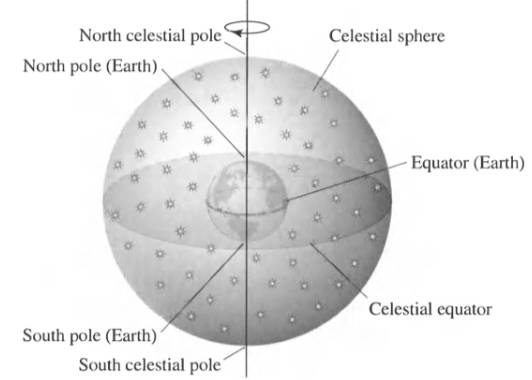
\includegraphics[width=6cm]{chapters/01/celestialsphere}
	\caption{天球,地球在中央,天球赤道和地球赤道共面。}
	\label{fig:celestialsphere}
\end{figure}


\begin{figure}[hbt]
  \centering
  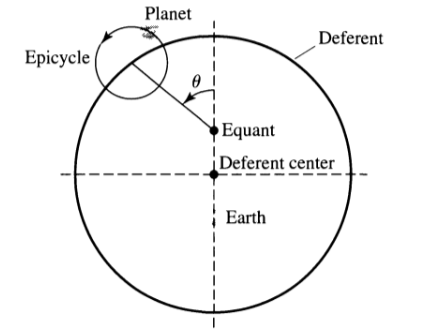
\includegraphics[width=6cm]{chapters/01/ptolemaicmodel}
  \caption{提出本轮、均轮、equant来解释{\bf 逆行运动}	}
  \label{fig:ptolemarcmodel}
\end{figure}

\section{日心说}
内行星:位于地球轨道以内的行星。相对于太阳最大的角间距称为{\bf 东、西大距},此时视亮度最大。

外行星:位于地球轨道以外的行星。亮度最大处称为照。

合:从地球上看,跑到太阳一侧,对于内行星,在太阳背后叫上合,在太阳前面叫下合

冲:从地球上看,跑到太阳反方向

会合周期(S):相邻两次冲或合(相对地球)的时间间隔

恒星周期(P):完成一次公转所需要的时间

\begin{displaymath}
  1/S=
  \begin{dcases}
  	1/P-1/P_{\oplus}\ \text{(内行星)} \\
  	1/P_{\oplus}-1/P\ \text{(外行星)}
  \end{dcases}
\end{displaymath}

\section{天球坐标}\label{sec:celestial}
\subsection{高度方位坐标系}
\begin{figure}[hbt]
  \centering
  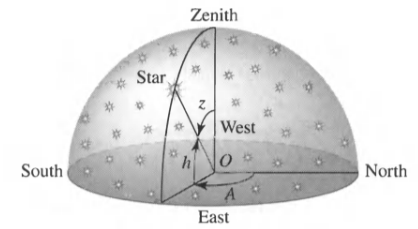
\includegraphics[width=6cm]{chapters/01/altitude}
  \caption{高度方位坐标系}
  \label{fig:altitude}
\end{figure}

高度角$h$:天体与水平面的夹角,如图\ref{fig:altitude}

天顶:观测者正上方

天顶距$z$:天体与天顶的夹角

方位角$A$:从某点的指北方向线(通常用子午线,即经线)起依顺时针(东)方向至目标方向线间的水平夹角

地球的自转轨道面(赤道面)和公转轨道面(黄道面)存在夹角(黄赤交角),因此在一年中太阳的直射点会发生变化,由此定义春分点、夏至点、秋分点、冬至点。

太阳时:太阳经过子午线的平均间隔(考虑地球自转)

恒星时:背景恒星经过子午线的平均间隔

\subsection{赤道坐标系}

\begin{figure}[hbt]
  \centering
  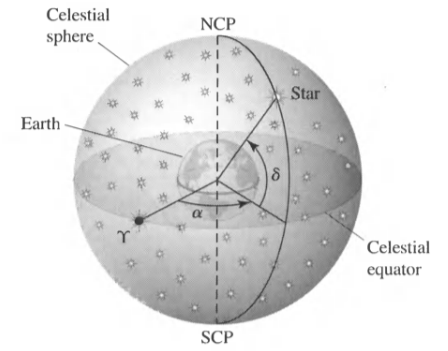
\includegraphics[width=6cm]{chapters/01/equatorial}
  \caption{赤道坐标系}
  \label{fig:equatorial}
\end{figure}
赤纬$\delta$:等价于纬度

赤经$\alpha$:自春分点依顺时针(东)方向至被测点所在时圈的时差,一周24小时等价于360$^\circ$,1h=15$^\circ$,1m=15$'$
,1s=15$''$

本地恒星时:观测者所在子午线的赤经

{\bf
进动(岁差)}会导致天体的赤经、赤纬发生变化(因为春分点发生变化),因此要确定一个特定的时期来确定春分点的变化,对赤道坐标作出修正
,这个时期被定义为2000年1月1日正午英国格林尼治的观测值(J2000.0)

\begin{align}
  \Delta\alpha &=M+N \sin\alpha \tan\delta \\
  \Delta\delta &=N\cos\alpha
\end{align}

其中

\begin{align}
  M &=1^\circ.2812323T+0.^\circ0003879T^2+0.^\circ0000101T^3 \notag \\
  N &=0^\circ.5567530T-0.^\circ0001185T^2-0.^\circ0000116T^3 \notag
\end{align}

其中$T$定义为

\begin{equation}
  T=(t-2000.0)/100
\end{equation}

其中$t$是当前时间,以年的分数来表示。

\subsection{自行}
天体本身通常具有相对太阳运动,其速度可分解为视向速度$v_r$和切向速度$v_\theta$,而切向速度会导致天体的坐标发生变化,这种运动被称为{\bf 自行}
\begin{displaymath}
  \mu\equiv{d\theta\over dt} ={v_\theta \over r}
\end{displaymath}

\begin{figure}[hbt]
  \centering
  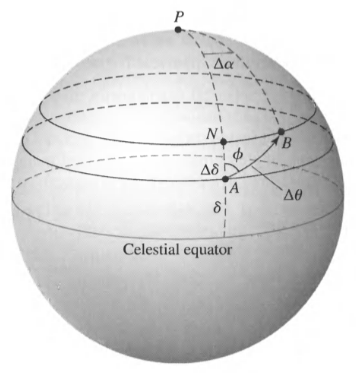
\includegraphics[width=6cm]{chapters/01/propermotion}
  \caption{自行示意图}
  \label{fig:proper}
\end{figure}


考虑到在天球上运动的几何关系如图\ref{fig:proper},且天体是沿位置角$\phi$运动,可以得到
\begin{align}
   \Delta\alpha &=\Delta\theta{\sin \phi \over \cos \delta}\\
   \Delta\delta &=\Delta\theta\cos\phi\\
   (\Delta\theta)^2 &=(\Delta\alpha\cos\delta)^2+(\Delta\delta)^2
\end{align}


\chapter{天体力学}
\section{牛顿力学}
牛顿三大定律+万有引力定律

联立动能和势能的关系$K=-U$,可得逃逸速度$v_{ves}=\sqrt{2GM/r}$

\section{开普勒定律}
在多体运动的研究中,使用{\bf 质心参考系}会更加方便,质心$\mathbf{R}\equiv {m_1 \mathbf{r}'_1+m_2
\mathbf{r}'_2 \over m_1+m_2} $可代替多体系统的整体运动情况,折合质量$\mu \equiv {m_1m_2 \over m_1
+m_2}$可表征系统的能量分布情况,因此两体的位移矢量$\mathbf{r_1}$和$\mathbf{r_2}$可表示为:
\begin{align}\label{eq:r}
  \mathbf{r_1} &=-{\mu\over m_1}\mathbf r\\[2mm]
  \mathbf{r_2} &=-{\mu\over m_2}\mathbf r
\end{align}

牛顿力学为开普勒定律提供了数学解释。
\subsection{开普勒第一定律}
{\bf 行星绕太阳运动的轨道是一个椭圆,太阳在椭圆的一个焦点上}。

\begin{equation}
  r={L^2/\mu^2 \over GM(1+e\cos\theta)}
  \label{eq:kepler1}
\end{equation}

式\ref{eq:kepler1}为极坐标下的圆锥曲线,{\bf 折合质量受引力作用绕质心运动的轨迹是圆锥曲线(抛物线、双曲线、椭圆)}。

\begin{equation}
  L=\mu\sqrt{GMa(1-e^2)}
\end{equation}

其中$L$在圆周运动($e=0$)时最大,抛物线运动($e\rightarrow 1$)时趋于0。

\subsection{开普勒第二定律}
{\bf 行星和太阳的连线在相同时间间隔内扫过的面积相等}。

\begin{equation}
  v^2=G(m_1+m_2)({2\over r}-{1\over a})
  \label{eq:kepler2}
\end{equation}


\subsection{开普勒第三定律}
{\bf (周期)平方(半长轴)反比律,或调和定律}

\begin{equation}
  P^2={4\pi^2 \over G(m_1+m_2)}a^3\;\text{国际单位制}
\end{equation}

方便起见,有时可写成:
\begin{equation}
  p^2={1\over (m_1+m_2)}a^3
  \label{eq:kepler3}
\end{equation}
其中$P$的单位是年,$a$的单位是AU,$m$的单位是太阳质量

\section{维里定律}
{\bf 对于引力束缚的平衡系统,平均动能总是平均势能的一半}
\begin{equation}
  -2\langle K \rangle=\langle U \rangle
  \label{virial}
\end{equation}


\chapter{光的连续谱}
\section{恒星视差}
恒星视差被用于距离测量,这种方法被称为{\bf 三角视差}

\begin{figure}[hbt]
  \centering
  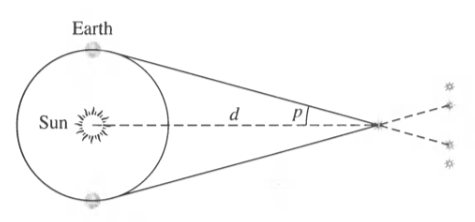
\includegraphics[width=6cm]{chapters/03/parallax}
  \caption{恒星视差,$d=1/p''\mathrm{pc}$}
  \label{fig:parallax}
\end{figure}

如图\ref{fig:parallax}所示,当地球运行到公转轨道的两端时,会观测到目标恒星的位置相对背景星空发生了变化,这种变化体现在天球坐标
(\autoref{sec:celestial})的变化上,即坐标差$p$,通过三角形几何关系,可以得到目标恒星的距离$d$,从而定义秒差距:
\begin{equation}
  d=1/p''\mathrm{pc}
\end{equation}

单位换算:$1\;\mathrm{pc}\approx
3.26\;\mathrm{ly}$,$1\;\mathrm{ly}\approx9.46\times10^{15}\;\mathrm m$

\section{星等}
古希腊的喜帕恰斯(Hipparchus)定义了{\bf 视星等}$m$,且天空最亮的恒星为$m=1$,肉眼看到最暗的恒星为$m=6$。现代观测设备能够定量精确地测量恒星的{\bf 辐射流量}$F$,发现相差5个星等对应辐射流量差100倍,于是得到关系:
\begin{equation}
  m_1-m_2=-2.5\log_{10}\left({F_1\over F_2}\right)
  \label{eq:magnitude}
\end{equation}

地球上测得的太阳的辐射流量称为{\bf 太阳辐照度},或太阳常数:$F={L_\odot \over 4\pi r^2}=1365\;\mathrm{W\;m^{-2}}$

视星等只能观测属性,无法表征恒星本身的发光能力,因此定义当恒星处于10pc处时的视星等为{\bf 绝对星等}$M$,可得到{\bf 距离模数}:
\begin{equation}
  m-M=5\log_{10}\left({d\over 10\;\mathrm{pc}}\right)
  \label{eq:module}
\end{equation}

{\bf \textcolor{red}{注:星等概念注意理解,才能灵活运用}}

\section{黑体辐射}
一个理想的发射源也应该吸收所有入射到其表面上的光,然后再以特征谱的形式辐射出来,这种理想发射源称为{\bf 黑体},相应的辐射称为{\bf 黑体辐射}
\begin{figure}[hbt]
  \centering
  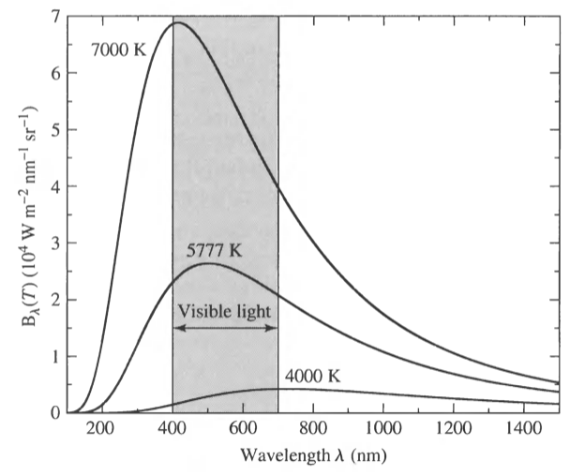
\includegraphics[width=6cm]{chapters/03/blackbody}
  \caption{黑体的光谱}
  \label{fig:blackbody}
\end{figure}

如图\ref{fig:blackbody}所示,黑体谱应该是覆盖全波段的连续谱,但是辐射强度随波长呈一定分布,峰值波长(频率)满足{\bf 维恩位移定律}:
\begin{equation}
  \lambda_\mathrm{max}T\approx0.0029\;\mathrm{m\;K}
\end{equation}

图\ref{fig:blackbody}的黑体谱可以用{\bf 普朗克公式}来描述:
\begin{equation}
  B_\lambda(T)={2hc^2/\lambda^5 \over e^{hc/\lambda kT}-1}
  \label{eq:planck}
\end{equation}

或频率形式:
\begin{equation}
  B_\upsilon (T)={2h\upsilon^3/c^2 \over e^{h\upsilon/kT}-1}
\end{equation}

黑体辐射的光度可用{\bf 斯特藩-玻尔兹曼定律}描述:
\begin{equation}
  L=4\pi R^2\sigma T^4_e
  \label{eq:stefan}
\end{equation}

尽管恒星并不是理想黑体,但是依然可以使用式\ref{eq:stefan}来定义恒星表面的{\bf 有效温度}$T_e$

\section{色指数}
一颗恒星全波段测量得到的星等称为{\bf 热星等(bolometric magnitudes)},记为$m_{bol}$和$M_{bol}$

观测时,往往使用滤光片来使特定波段的光透过,从而精确测量恒星的颜色,滤光片的带宽和中心频率由制作时随需求确定,但有时也用统一标准:
\begin{itemize}
  \item U,紫外星等,中心波长365\;nm,有效带宽68\;nm
  \item B,蓝光星等,中心波长440\;nm,有效带宽98\;nm
  \item V,可见光星等,中心波长550\;nm,有效带宽89\;nm
\end{itemize}

一颗恒星不同波段的星等之差称为{\bf 色指数(color index)},如色指数$B-V$的值越小,说明恒星在$B$波段越亮

热星等和可见光星等的差称为{\bf 热改正(bolometric correction) $BC$}:
\begin{equation}
  BC=m_\mathrm{bol}-V=M_\mathrm{bol}-M_V
  \label{eq:bc}
\end{equation}

现实中无法测量恒星的热星等,但是可以通过式\ref{eq:bc}将光星等+热改正来得到热星等

由式\ref{eq:magnitude}可推得对应波段的星等:
\begin{equation}
  U=-2.5\log_{10}\left(\int_0^\infty F_\mathrm\lambda S_U d\lambda\right)+C_U
\end{equation}

其中$S_U$是响应函数,用于描述入射光的比率,和望远镜的镜面反射率有关,计算时可考虑在有效带宽内为1,有效带宽外为0;$C_U$是一个常数。

上式类比到其他波段可得色指数:
\begin{equation}
  U-B=-2.5\log_{10}\left({B_{365}\Delta\lambda_U \over B_{440}\Delta\lambda_B}\right)+C_{U-B}
\end{equation}

\begin{figure}[hbt]
  \centering
  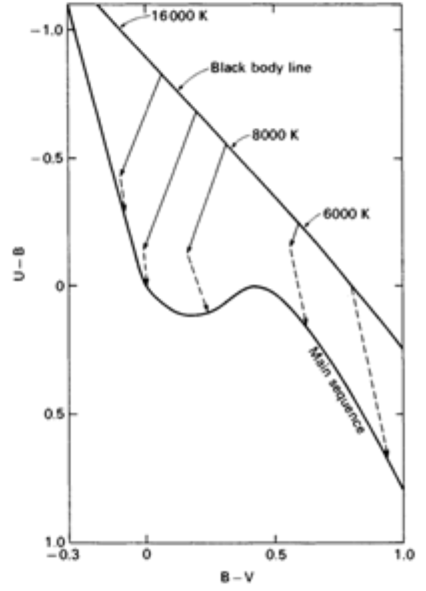
\includegraphics[width=6cm]{chapters/03/CC}
  \caption{双色图,从中可以看出恒星并不是严格的黑体谱,一些特定的发射线会导致特定波段的光强偏离黑体谱,从而出现图中的虚线和实线(氢原子巴尔末线系)箭头所导致的偏差。}
  \label{fig:cc}
\end{figure}

\chapter{狭义相对论}
\section{洛伦兹变换}
\subsection{基本假设}
\paragraph{相对性原理}
物理定律在所有惯性参考系中都相同
\paragraph{光速不变}
光在真空中的传播速度恒为$c$,与观测者(光源)的运动情况无关
\begin{align}
  x' &={x-ut \over \sqrt{1-u^2/c^2}}\\
  y' &=y\\
  z' &=z\\
  t' &={t-ux/c^2 \over \sqrt{1-u^2/c^2}}
\end{align}

\textcolor{red}{{\bf 注:运动是相对的},运用洛伦兹变换时应注意对应坐标系,$x$对应的是相对静止测量的坐标系,如在运动火车上测量火车上的坐标;$x'$对应相对运动测量的坐标系,如在运动火车上测量地面上的坐标}

\section{时空观}
狭义相对论提出了{\bf 同时的相对性},以及对应的\textbf{时间延缓}和\textbf{长度收缩}效应:
\begin{align}
  \Delta t_\mathrm{moving}&={\Delta t_\mathrm{rest} \over \sqrt{1-u^2/c^2}}\\
  L_\mathrm{moving}&=L_\mathrm{rest}\sqrt{1-u^2/c^2}
\end{align}

\textcolor{red}{{\bf 注:}同上,注意下标所对应的都是相对测量的运动情况,计算时分清楚对应的坐标系}

\begin{figure}[hbt]
  \centering
  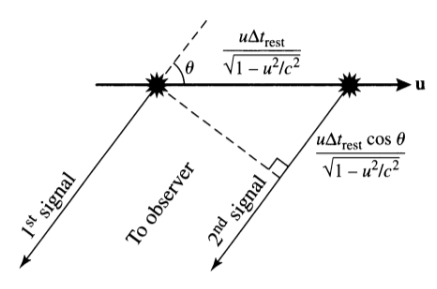
\includegraphics[width=6cm]{chapters/04/dopper}
  \caption{相对论性多普勒频移}
  \label{fig:doppler}
\end{figure}

如图\ref{fig:doppler}所示,由于光源的视向运动的光性差,考虑狭义相对论的时间延缓效应,会导致接受者所观测到的光频发生变化
\begin{equation}
  \upsilon_\mathrm{obs}={\upsilon_\mathrm{rest}\sqrt{1-u^2/c^2}\over 1+v_r/c}
  \label{eq:doppler}
\end{equation}

光源朝向观测者的运动会导致蓝移,远离观测者的运动会导致红移,频移的程度可以用\textbf{红移参数}$z$来描述:
\begin{equation}
  z\equiv{\lambda_\mathrm{obs}-\lambda_\mathrm{rest}\over \lambda_\mathrm{rest}}={\Delta\lambda \over \lambda_{rest}}=\sqrt{{1+v_r/c \over 1-v_r/c}}-1
\end{equation}

相对论效应还会导致在运动坐标系中观测到的速度发生变化:
\begin{align}
  v_x' &={v_x-u \over 1-uv_x/c^2}\\[2mm]
  v_y' &={v_y\sqrt{1-u^2/c^2} \over 1-uv_x/c^2}\\[2mm]
  v_z' &={v_z\sqrt{1-u^2/c^2} \over 1-uv_x/c^2}
\end{align}

由于观测速度的变化主要体现在坐标系运动方向上,因此合速度的方向也会发生变化$\sin\theta={v_y /v}=\gamma^{-1}$,当相对论效应足够强时,$\theta\sim\gamma^{-1}$,即速度会被收束在二倍的$\gamma^{-1}$的张角内,这被称为\textbf{头灯效应(headlight effect)},如图\ref{fig:beaming}所示,同步辐射因此而显现出偏振态

\begin{figure}[hbt]
  \centering
  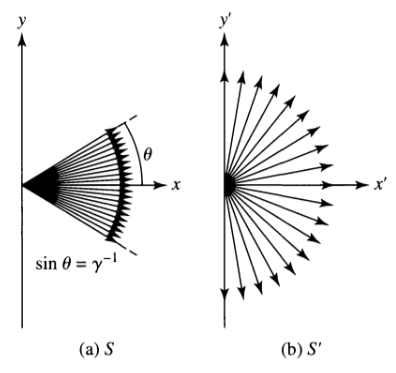
\includegraphics[width=6cm]{chapters/05/beaming}
  \caption{头灯效应}
  \label{fig:beaming}
\end{figure}


\section{相对论动量和能量}
由于要满足相对论性原理,即所有惯性系下动量都应相同,因此定义\textbf{相对论性动量}
\begin{equation}
  \mathbf p=\gamma m \mathbf v
\end{equation}

以及相对论性动能:
\begin{equation}
  K=\underbrace{ \gamma mc^2}_\text{相对论性总能量}-\underbrace{mc^2}_\text{静能量}=mc^2(\gamma-1)
\end{equation}

相对论性总能量还可以写为(作业题):
\begin{equation}
  E^2=p^2c^2+m^2c^4
\end{equation}

该式可适用于计算无质量的粒子,如光子的总能量

\chapter{光与物质的相互作用}
\section{光谱}
通过恒星光谱的多普勒频移可以计算恒星的视向速度(式\ref{eq:doppler})。

现代天文学家使用光谱仪来获取恒星的光谱,光谱的作用是把接收到的恒星的复合光按照不同波长展开,目前大多使用衍射光栅来实现。

越好的光谱仪能够将光谱展的越开,展现更加精细的光谱结构,因此定义光谱仪的分辨本领:
\begin{equation}
  \Delta\lambda={\lambda \over nN}
\end{equation}

\paragraph{基尔霍夫定律}\label{kirchhoffs}
\begin{itemize}
  \item 一团热的稠密气体或固体能够产生没有暗线的连续光谱
  \item 一团热的稀薄气体能够产生明亮的光谱线(发射线),发射线频率与跃迁的能级差对应
  \item 一团冷的稠密气体挡在一个产生连续光谱的光源前,能够在连续谱上产生对应原子能级的暗线(吸收线),吸收线频率与跃迁的能级差对应
\end{itemize}

基尔霍夫定律中的\textbf{冷}与\textbf{热}都是相对而言。

\section{光子}
\paragraph{光电效应}
当光照射在金属表面,会从金属表面激发出电子的过程

由于存在原子能级,只有频率大于\textbf{截止频率}的光子才能够激发出电子,在激发出电子的基础上,增加光强只能增加激发出的电子数目,增加入射光的频率能够增加电子的出射动能:
\begin{equation}
  K_\mathrm{max}=E_\mathrm{photon}-\underbrace{\phi}_\text{\clap{金属的溢出功(电子的最小结合能)}}=h\upsilon-\phi={hc \over \lambda}-\phi
\end{equation}

\paragraph{康普顿效应}
高能光子与自由电子发生碰撞,散射光子能量降低的过程,如图\ref{fig:compton}。

\begin{figure}[hbt]
  \centering
  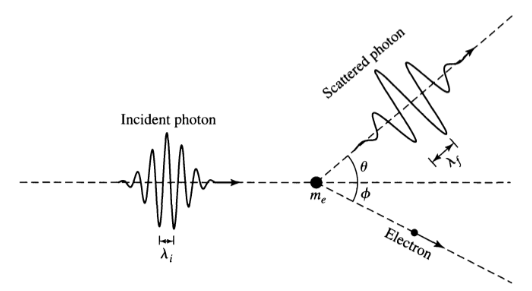
\includegraphics[width=10cm]{chapters/05/compton}
  \caption{康普顿散射示意图}
  \label{fig:compton}
\end{figure}

\section{玻尔的原子模型}
玻尔的原子模型指出,\textbf{原子核周围存在不同的轨道能级,电子位于固定能级上,能级跃迁需要吸收或释放相应能量(光子)},如图\ref{fig:atom}。

通过假设原子核与电子通过库仑力相互作用,以及角动量量子化,得到代表轨道半径的\textbf{玻尔半径}:
\begin{equation}
  r_n={4\pi \epsilon_0 \hbar^2 \over \mu e^2}n^2=a_0n^2
\end{equation}

以及轨道能级:
\begin{equation}
  E_n=-{\mu e^4\over 32\pi^2\epsilon^2\hbar^2}{1\over n^2}=-13.6\;\mathrm{eV}{1\over n^2}
\end{equation}

其中$n$为主量子数,表征原子的每个轨道。

\begin{figure}
  \centering
  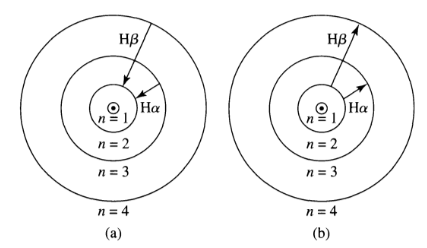
\includegraphics[width=10cm]{chapters/05/atom}
  \caption{玻尔的氢原子模型的巴尔末线系(a)发射线(b)吸收线}
  \label{fig:atom}
\end{figure}

玻尔的模型能够较好的解释实验得到的氢原子发射谱线,并可以计算得到氢原子的基态能量$E_1=-13.6\;\mathrm{eV}$,通过计算不同能级的能量差,可以得到轨道跃迁对应的光子波长:
\begin{equation}
  E_\mathrm{photon}=E_\mathrm{high}-E_\mathrm{low}\notag
\end{equation}

或写为
\begin{equation}
  {hc \over \lambda}=-{\mu e^4\over 32\pi^2\epsilon^2\hbar^2} \left({1\over n_\mathrm{high}^2}- {1\over n_\mathrm{low}^2}\right)
\end{equation}

电子在$n=1$与更高能级的相互跃迁所产生的一系列谱线称为\textbf{莱曼线系},用符号Ly表示,$n=1$和$n=2$之间跃迁为Ly$\alpha$,$n=1$和$n=3$之间跃迁为Ly$\beta$,以此类推。

同理,电子在$n=2$与更高能级的相互跃迁所产生的一系列谱线称为\textbf{巴尔末线系},图\ref{fig:atom}所示为波尔模型的氢原子的巴尔末线系,用符号H表示,$n=2$和$n=3$之间跃迁为H$\alpha$,$n=2$和$n=4$之间跃迁为H$\beta$,以此类推。其他线系如图\ref{fig:level}

\begin{figure}[hbt]
  \centering
  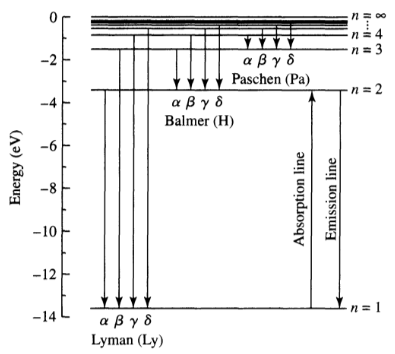
\includegraphics[width=7cm]{chapters/05/level}
  \caption{氢原子的能级跃迁图,包括莱曼、巴尔末、帕邢线系}
  \label{fig:level}
\end{figure}

\section{量子力学}
\subsection{物质波}
德布罗意将\textbf{波粒二象性}推广到所有粒子,提出了物质波,并给出了相应的波长和频率的表达式:
\begin{align}
  \upsilon &= {E\over h}\\[2mm]
  \lambda &= {h\over p}
\end{align}

这种波长和频率被称为德布罗意波长和频率,实际上该式可以推广到一切物体,如计算得到\textbf{一个慢跑的人类的德布罗意波长}$\lambda\sim3.16\times10^{-36}\;\mathrm m$,远小于观测极限,因此可以忽略不计。

\subsection{海森堡的不确定性原理}\label{uncertainty}
不确定性原理指出波粒二象性的内禀属性,当观测时,粒子的位置确定,则动量的不确定会变大,反之亦然。

\begin{equation}
  \Delta x \;\Delta p\geq{1\over2}\hbar
\end{equation}

也可以近似表达为
\begin{equation}
  \Delta x \;\Delta p\approx \hbar
\end{equation}

同时对应能量和时间也存在不确定性关系:
\begin{equation}
  \Delta E \;\Delta t\approx \hbar
\end{equation}

\paragraph{量子隧穿}
由于波粒二象性,粒子以几率波的形式分布在空间中,对于一些比较高的势垒,从能量角度看可能无法穿过,但是实际上波函数已经穿透,只是透过之后很快衰减了。但是波函数透过代表就有一定几率粒子能够穿过势垒,发生量子隧穿。

\subsection{薛定谔方程和量子力学原子模型}
为了描述粒子的波动性,薛定谔提出\textbf{薛定谔方程}来描述波函数,同时发现仅仅通过主量子数$n$无法完全描述原子的能级,提出
\begin{itemize}
  \item \textbf{角量子数}$\ell$,描述原子的角动量$L=\sqrt{l(l+1)}\hbar$,$\ell=0,1,2,3,4,5$等分别对应轨道$s,p,d,f,g,h$等。
  \item \textbf{磁量子数}$m_\ell$,描述原子角动量$z$分量$L_z=m_\ell \hbar$,$m_\ell$为$-\ell$和$+\ell$间的任意整数。
\end{itemize}

不同的轨道量子数$\ell$和$m_\ell$但具有相同的主量子数(相同能量)称为\textbf{简并}。

同时电子还具有\textbf{自旋量子数}$m_s=\pm{1\over2}$,用来表征电子内禀的自旋角动量$z$分量$S_z=m_s \hbar$。

电子由于具有不同的自旋,在磁场中会产生不同的能级,导致谱线会分裂,这种现象称为\textbf{塞曼效应},对于频率为
\begin{equation}
  \upsilon=\upsilon_0\qquad \text{和}\qquad \upsilon_0\pm{eB\over 4\pi\mu}
\end{equation}

\paragraph{泡利不相容原理}
两个电子不能具有完全相同的一组(4个)轨道量子数。

实际上泡利不相容原理适用于所有费米子(电子、中子等构成物质的基本粒子),而玻色子(光子等构成能量的基本粒子)可以具有完全相同的能量状态,且费米子的自旋角动量只能是${1\over2}\hbar$的奇数倍,而玻色子的自旋角动量是$\hbar$的整数倍。

\chapter{望远镜}
\section{基础光学}
\paragraph{斯涅尔定律}
表示折射的规律,$n_{1\lambda}\sin\theta_1=n_{2\lambda}\sin\theta_2$

\paragraph{透镜公式}
${1\over f_\lambda}=(n_\lambda-1)\left({1\over R_1}-{1\over R_2} \right)$,其中$R_1$和$R_2$是折射面的曲率,凸面为正,凹面为负。

透镜的\textbf{放大本领}可以用底片放大率(plate scale)表示
\begin{equation}
  {d\theta\over dy}={1\over f}
\end{equation}

可得透镜的焦距越大,相同角间距的两点能够呈现更大的像。但事实上无法通过简单的提高焦距来提升望远镜的性能,因为极小的角间距会产生衍射,因此存在一个受波长$\lambda$和光圈大小$D$(或孔距)限制的最小分辨角,表征透镜的\textbf{分辨本领}(瑞利判据):
\begin{equation}
  \theta_\mathrm{min}=1.22{\lambda \over D}
\end{equation}

\paragraph{视宁度}
望远镜显示图像的清晰度,取决于大气的湍流活动引起光线折射的程度。

\paragraph{像差}
透镜和镜面系统所带来的图像畸变称为像差(aberrations),包括
\begin{itemize}
  \item 色差,折射式望远镜由于折射率与波长有关,不同波长的光汇聚在不同焦平面上,可通过增加改正透镜来降低影响
  \item 球差,球面镜的边缘比中心具有更强折射能力,使得平行光无法汇聚在一点,可通过设计(抛物面)消除
  \item 彗差,抛物面镜对偏离光轴的光源的入射光不能汇聚在一点上,即焦距与入射光与光轴夹角有关,彗尾状的像而得名,可通过选择合适的表面曲率降低影响
  \item 散光,透镜或镜面成像不在预定焦平面上,属于设计缺陷
  \item 场曲,成像不在平面,而是在曲面上
  \item 场变,底片放大率与到光轴的距离相关
\end{itemize}

望远镜的\textbf{获取光线的本领}称为照度$J\propto 1/F^2$,其中\textbf{焦比}$F\equiv f/D$。

\section{望远镜}
\paragraph{折射式}——叶凯士天文台
\begin{itemize}
  \item 角放大率$m=f_\mathrm{obj}/f_\mathrm{eye}$
  \item 产生色差
  \item 边缘支撑时间久了会变形
  \item 热响应慢
  \item 容易有设计缺陷
\end{itemize}

\paragraph{反射式}——卡塞格林望远镜、施密特望远镜
\begin{itemize}
  \item 只需要注意维护反射面
  \item 主动光学
  \item 各种设计
\end{itemize}

\paragraph{主动光学(active optics)}
观测时温度变化和望远镜移动会导致镜面的形变,主动光学就可以通过在镜面后增加活塞改变镜面曲率,或每隔几分钟调整望远镜朝向来修正

\paragraph{自适应光学(adaptive optics)}
有了主动光学,观测误差来源主要就在大气湍流,自适应光学通过计算机可在曝光同时快速修正,通常可以在光路中插入一个小透镜,调整小透镜的曲率来调整焦点位置

\paragraph{望远镜支架}——赤道仪式、高度-方位式

\paragraph{射电望远镜}——FAST、VLA,
可通过增大面积(综合孔径)和干涉(VLBI)的方式提高分辨率。
\newline

由于大气窗口,红外、紫外、x射线和伽马射线的望远镜需要发射到太空。
\paragraph{红外望远镜}——Spitzer、Hershel

\paragraph{紫外望远镜}——IUE国际紫外望远镜、EUVE极紫外探测器

\paragraph{x射线望远镜}——Chandra、XMM-Newton

\paragraph{伽马射线望远镜}——Fermi、悟空

\part{The Nature of Stars}
\chapter{双星系统和恒星参数}
\section{双星分类}
\begin{itemize}
  \item 光学双星(optical double),只是观测看起来在一块,相互之间不受引力束缚
  \item 目视双星(visual binary),观测上能够直接分辨出两颗星
  \item 天测双星,伴星可能由于太暗不可见,但是可以从主星的运动情况分辨存在伴星
  \item 食双星,绕转轨道沿视线方向,会相互遮掩,能够观测到周期性的光度变化
  \item 光谱双星,具有独立、可分辨的光谱,可通过光谱分辨的双星,两颗星的光谱分别红移和蓝移
  \item 分光双星,周期短,可通过光谱的周期性红移分辨
\end{itemize}

以上分类并不相互独立,一个双星系统可以符合多种分类。

\section{目视双星测定质量}
第二章中提到多体运动可以使用质心参考系来研究,而在质心参考系中,位移矢量与质量存在关系(式\ref{eq:r}):
\begin{equation}
  {m_1\over m_2}={r_2\over r_1}={a_2\over a_1}
\end{equation}

上式$a$为椭圆轨道的长半轴,如果假定地球到该双星系统的距离$d$,且双星轨道平面垂直于视线,则可转化为质量$m$与角间距$\alpha$的关系:
\begin{equation}
  {m_1\over m_2}={a_2\over a_1}={\alpha_2 d\over \alpha_1 d}={\alpha_2\over \alpha_1}
\end{equation}

若双星轨道平面不垂直于视线,与垂直面存在倾角$i$,则上式变为
\begin{equation}
  {m_1\over m_2}={\alpha_2 \cos{i}\over \alpha_1\cos{i}}={\widetilde \alpha_2 \over \widetilde \alpha_1}
  \label{eq:binary1}
\end{equation}

同时考虑开普勒第三定律(式\ref{eq:kepler3})可得
\begin{equation}
  m_1+m_2={4\pi^2 \over G}{(\alpha d)^3 \over P^2}={4\pi^2\over G}\left({d\over \cos i}\right)^3{\widetilde \alpha^3\over P^3}
  \label{eq:binary2}
\end{equation}

其中$\widetilde \alpha=\widetilde \alpha_1+\widetilde \alpha_2$,结合式\ref{eq:binary1}和式\ref{eq:binary2}可得两颗恒星的质量。

\section{食双星和分光双星}
这种情况下一般只能得到一颗恒星的视向速度和周期,利用质心参考系的性质和开普勒第三定律,可以得到\textbf{质量函数}
\begin{equation}
  {m^3_2\over (m_1+m_2)^2}\sin^3 i={P\over 2\pi G}v^3_{1r}
\end{equation}

上式右边全是可观测量,若只能探测到一颗恒星的视向速度,则可以用上式得到$m_2$的下限,若可以探测到两颗恒星的视向速度,则结合下式可以计算两颗恒星的质量
\begin{equation}
  {m_1\over m_2}={v_{2r}/ \sin{i}\over v_{1r}\sin{i}}={v_{2r} \over v_{1r}}
\end{equation}

由于食双星和分光双星需要双星绕转平面与视线平行,才能够观测到足够的视向速度,所以通常可取$\langle\sin^3 i\rangle\simeq2/3$

\subsection{利用日食确定半径和温度比}
\begin{figure}[hbt]
  \centering
  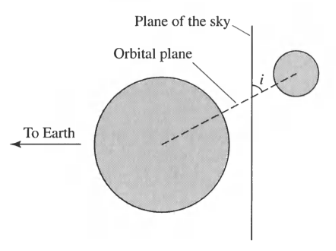
\includegraphics[width=6cm]{chapters/07/eclipse1}
  \caption{日食示意图,倾角$i$应接近90$^\circ$}
  \label{}
\end{figure}

\begin{figure}[hbt]
  \centering
  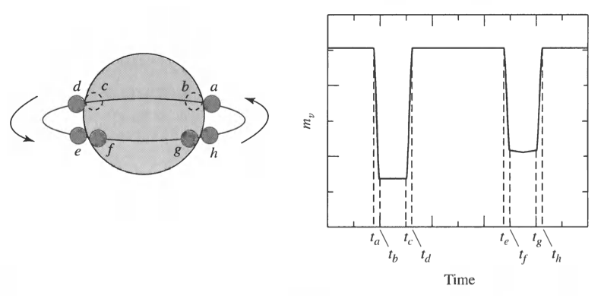
\includegraphics[width=12cm]{chapters/07/eclipse2}
  \caption{$i=90^\circ$(完全日食)的光变曲线,假设小恒星比大恒星更热}
  \label{}
\end{figure}

\begin{figure}[hbt]
  \centering
  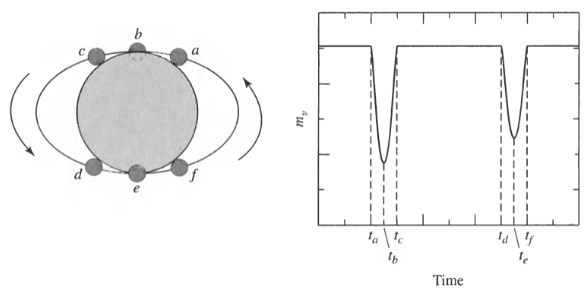
\includegraphics[width=12cm]{chapters/07/eclipse3}
  \caption{部分日食的光变曲线,假设小恒星比大恒星更热}
  \label{}
\end{figure}

由上图的光变曲线示意图可以得到两颗恒星的半径:
\begin{align}
  r_s&={v\over 2}(t_b-t_a)\\
  r_\ell &={v\over 2}(t_c-t_a)=r_s+{v\over 2}(t_c-t_b)
\end{align}

通过恒星半径以及斯特藩-玻尔兹曼公式(式\ref{eq:stefan}),可以得到温度$T$与亮度$B$的关系:
\begin{equation}
  {B_0-B_p\over B_0-B_s}=\left({T_e\over T_\ell}\right)^4
\end{equation}

其中$B_0$为两星分开的最大亮度,$B_p$为光变曲线的最小值,$B_s$为光变曲线的次极小值。

\chapter{恒星光谱的分类}
\subsection{恒星光谱型}
\paragraph{哈佛分类法}
通过斯特藩-玻尔兹曼定律可以确定恒星的有效温度,根据有效温度由高到低可将恒星分为``O B A F G K M'',中间还具体细分为十级(如A0-A9),由于天文学界一开始误认为恒星也是按照这样的顺序来演化的,因此靠左的类型又称为\textbf{早型星},靠右的类型又称为\textbf{晚型星}。

\paragraph{MK光度级}
实际上是通过光谱分辨恒星的演化阶段,对应罗马字母I到V,将I型定义为超巨星,V型定义为主序星,后来又补充了VI型为亚矮星,VII型为白矮星。对于单个恒星的演化,主序、巨星、超巨星阶段的光度随半径增加(参考\ref{sec:evolution}节),而半径增加会导致恒星表面引力减弱,压强减小,从而压强增宽机制会减弱,产生的谱线宽度会较小,因此,可以通过谱线宽度来确定恒星的光度。\mbox{}\\

上述两种光谱分类结合使用可以分别确定恒星的演化阶段和温度,从而在赫罗图上可以读出对应的光度,并根据视星等进一步计算出恒星的距离,这种测距方法称为\textbf{分光视差}。

\paragraph{麦克斯韦-玻尔兹曼速率分布}
描述在热平衡系统下,具有不同速率的粒子的数量分布
\begin{equation}
  n_v dv=n\left({m\over 2\pi k T}\right)^{3/2}e^{-mv^2/2kT}4\pi v^2 dv
  \label{eq:maxwell}
\end{equation}

\paragraph{玻尔兹曼方程}
描述处于不同激发态的原子数量比
\begin{equation}
  {N_b\over N_a}={g_b e^{-E_b/kT}\over g_a e^{-E_a/kT}}={g_b\over g_a}e^{-(E_b-E_a)/kT}
  \label{eq:boltzmann}
\end{equation}

其中$g_b$为$b$能级的简并度(有多少量子态具有相同能量),$E_b$为$b$能级的能量。

\paragraph{萨哈方程}
描述不同电离态的原子数量比
\begin{equation}
  {N_{i+1}\over N_i}={2Z_{i+1}\over n_e Z_i}\left({2\pi m_e kT\over h^2}\right)^{3/2} e^{-\chi_i/kT}
  \label{eq:saha}
\end{equation}

以及等价形式:
\begin{equation}
  {N_{i+1}\over N_i}={2kTZ_{i+1}\over P_e Z_i}\left({2\pi m_e kT\over h^2}\right)^{3/2} e^{-\chi_i/kT}
\end{equation}

其中$Z_i$为电离态为$i$的离子的配分函数:
\begin{equation}
  Z={\sum_{j=1}^\infty g_j e^{-(E_j)/kT}\over e^{-(E_1)/kT}}=g_1 {N\over n_1}
\end{equation}

从公式上看,配分函数其实是总原子数与基态原子数之比乘以基态简并度,描述的是\textbf{原子可能的状态数之和}。由于电离涉及电离能,不同能级的原子需要的电离能不同,同时并不是所有原子都处于基态,因此萨哈方程中利用基态电离能,但是乘以配分函数就可以考虑不同激发态的平均电离能。

\subsection{赫罗图}
\begin{figure}[hbt]
  \centering
  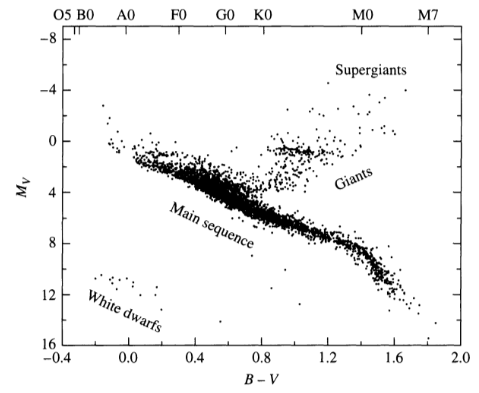
\includegraphics[width=14cm]{chapters/08/HRD}
  \caption{赫罗图}
  \label{}
\end{figure}

\chapter{恒星大气}
\paragraph{光强和辐射流量关系}
\begin{equation}
  F=\int I \cos\theta d\Omega=\int d\phi\int I \cos\theta\sin\theta d\theta =\sigma T^4
\end{equation}

\paragraph{能量密度}
\begin{equation}
  u={1\over c}\int I d\Omega=aT^4
\end{equation}

\paragraph{辐射压}
\begin{equation}
  P_\mathrm{rad}={2F \cos{\theta}\over c}={1\over3}aT^4={1\over 3}u
\end{equation}

\section{恒星不透明度}
前文提到恒星并不是理想黑体,产生的光谱也就不是严格的黑体谱,我们所观测到的恒星光谱主要来自恒星的光球层,但是恒星大气中存在的各种金属(天文中指比氢、氦重的元素)也会产生相应的谱线(参见\ref{kirchhoffs}节基尔霍夫定律)。

对于恒星的温度,我们也有多种定义:
\begin{itemize}
  \item 有效温度,通过斯特藩-玻尔兹曼定律(\ref{eq:stefan}),即发光能力来定义
  \item 激发温度,通过玻尔兹曼方程(\ref{eq:boltzmann}),即原子能级分布来定义
  \item 电离温度,通过萨哈方程(\ref{eq:saha}),即原子电离情况来定义
  \item 动力学温度,通过麦克斯韦-玻尔兹曼分布(\ref{eq:maxwell}),即粒子速率分布来定义
  \item 色温度,通过普朗克公式(\ref{eq:planck}),即恒星连续谱与黑体谱拟合来定义
\end{itemize}

其中有效温度是我们最常使用的,而其他温度只在恒星中的一些特殊区域应用,尽管这些温度定义不同,但是对于一团处于\textbf{热力学平衡}的理想气体,它们都是相同的。

\paragraph{热力学平衡}
不受外界作用的条件下,系统能够长久保持而不会发生变化的一种热力学状态,即内部能量产生与释放速率相等


然而,恒星并不是完全处于热力学平衡,不同位置的温度并不相同。但是如果处于\textbf{局部热力学平衡},即在粒子或光子的\textbf{平均自由程}(自由运动不与其他粒子发生相互作用的平均距离)内,温度变化很小,我们可以认为该区域处于相同温度。

对于光子来说,其平均自由程为:
\begin{equation}
  \ell={1\over \kappa_\lambda \rho}={1\over n \sigma_\lambda}
\end{equation}

其中$\kappa_\lambda$和$\sigma_\lambda$分别是不透明度(吸收系数)和散射截面,大小都与波长相关。

由于不能单纯地依靠光通过的距离来评估其衰减程度,因为相同距离,不同介质对光有不同的吸收效果,因此定义\textbf{光深$\tau_\lambda$来描述光子在传播过程中的平均碰撞次数}:
\begin{equation}
  \tau_\lambda=\int^s_0{ds\over \ell}=\int_0^s\kappa_\lambda\rho\,ds
\end{equation}

对于一定尺度的介质,$\tau\gg1$为光厚介质,$\tau\ll1$为光薄介质。

\paragraph{不透明度的来源}
\begin{itemize}
  \item 束缚-束缚跃迁(bound-bound transitions),光子如果能量与原子能级差吻合,会被电子吸收,跃迁到高能级
  \item 束缚-自由吸收(bound-free absorption),光子能量足够大时,能够直接电离电子,使电子进入自由态,此为光致电离。典型的例子是\textbf{巴尔末跳变},由于电子最终被电离,因此吸收光子的频率不像束缚-束缚跃迁要满足能级差,第一激发态的电子会对大于电离能(波长小于364.6\;nm)的光子全吸收,该区域谱线强度整体下降,如图\ref{fig:balmerjump}。
  \item 自由-自由吸收(free-free absorption),在离子附近的自由电子可以吸收光子,从能量较低的自由态进入能量更高的自由态,这是轫致辐射的逆过程
  \item 电子散射,与自由电子发生汤姆孙散射
\end{itemize}

\begin{figure}[hbt]
  \centering
  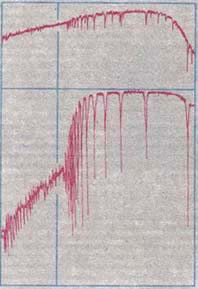
\includegraphics[width=4cm]{chapters/09/balmerjump}
  \caption{巴尔末跳变。图中蓝线对应波长364.6\;nm,氢的巴尔末线系的波长}
  \label{fig:balmerjump}
\end{figure}

由于不透明度和波长与介质有关,为了研究简便,我们通常会使用\textbf{罗斯兰平均不透明度}来替代,即对全波段的不透明度做加权平均,使其只对介质本身依赖
\begin{equation}
  {1\over \bar\kappa} \equiv{\displaystyle\int_0^\infty {1\over \kappa_\upsilon}{\partial B_\upsilon(T)\over \partial T}\,d\upsilon \over \displaystyle\int_0^\infty{\partial B_\upsilon(T)\over \partial T}\,d\upsilon}
\end{equation}

\section{辐射转移}
\subsection{光子辐射过程}
电子吸收光子会跃迁到高能级,但在高能级并不稳定,一段时间之后还会再落回低能态,这会伴随着辐射光子,因此光在经过介质时,\textbf{介质既会吸收光子也会辐射光子}。因此定义了发射系数$j_\lambda$,并用\textbf{辐射转移方程}来描述光强变化:
\begin{equation}
  {dI_\lambda \over d\tau_\lambda}=S_\lambda-I_\lambda
\end{equation}

其中$S_\lambda={j_\lambda\over \alpha_\lambda}$为原函数,若为常数,可得到方程特解:
\begin{equation}
  I_\lambda(\tau_\lambda)=\underbrace{I_{\lambda,0}e^{-\tau_\lambda}}_\text{入射光本身的衰减}+\underbrace{S_\lambda(1-e^{-\tau_\lambda})}_\text{介质对光强的净效果(吸收和辐射)}
\end{equation}

在局部热平衡的情况下,原函数$S_\upsilon=B_\upsilon$,即黑体辐射。

如果假设光子的传播方向时随机的,散射方向也是随机的,那么可以认为光子传播过程是\textbf{随机游走}过程,如果光子不被吸收,只被散射,它要穿过厚度为$d$的介质会被散射$N=d^2/\ell^2$次。

\paragraph{爱丁顿近似下的温度垂直分布}
\begin{equation}
  T^4={3\over 4}T_e^4\left(\tau_\upsilon+{2\over3}\right)
\end{equation}

其中$T_e$为有效温度,可以发现当$\tau_\upsilon=2/3$时,$T=T_e$,也就是说我们能看到的最深的光是来自恒星表面以下2/3光深处(表面$\tau_\upsilon=0$)。

\subsection{光谱线轮廓}
如果光子被吸收,就会恒星的连续谱中产生如图\ref{fig:spectrum}的谱线,被吸收的越多,则产生的``凹陷''越深,谱线越强,因此为了定量衡量谱线强度,定义\textbf{等值宽度}:
\begin{equation}
  W=\int{\displaystyle F_c-F_\lambda \over \displaystyle F_c}\,d\lambda
\end{equation}

即如图\ref{fig:spectrum}中定义一个矩形,高度和边缘相同,面积和``凹陷''面积相同,对应宽度即为等值宽度。

\begin{figure}[hbt]
  \centering
  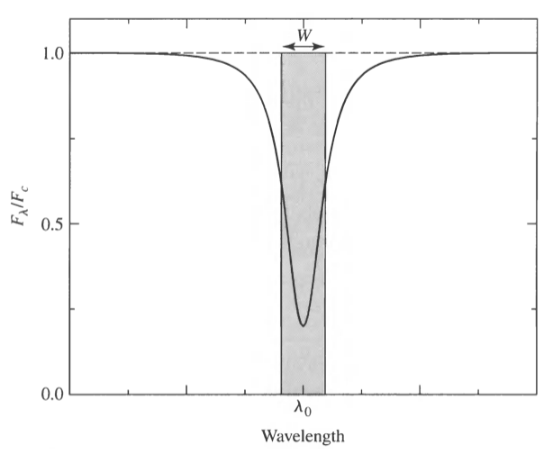
\includegraphics[width=10cm]{chapters/09/spectrum}
  \caption{典型的光谱线轮廓}
  \label{fig:spectrum}
\end{figure}

\subsection{谱线增宽机制}
前面讲过(\ref{kirchhoffs}节),电子能级跃迁才会在产生谱线,且谱线频率与跃迁的能级差相对应,那么谱线应该是一根严格的线,但是实际中会有几个主要机制会使谱线增宽:
\begin{itemize}
  \item \textbf{自然增宽},由于海森堡不确定性原理(\ref{uncertainty}节),原子在激发态上只能存在短暂瞬间,即在某能级的时间间隔$\Delta t$很小,因此对应的能级就无法精确测量,存在的误差$\Delta E\approx\hbar/\Delta t$就会较大,也就导致激发出的光子频率不是精确值,从而谱线产生增宽。
  \item \textbf{多普勒增宽},由于原子处于热运动,在发射光子时会产生多普勒频移,从而增宽
  \item \textbf{碰撞增宽(压强增宽)},碰撞会使激发态电子的寿命发生变化,本质与自然增宽相似
\end{itemize}

\chapter{恒星内部}
\section{描述恒星模型的方程}
研究恒星时,为了简便起见,我们通常把恒星看成是球对称分布的,因此只要研究简单的径向一维模型即可,然后辅以一下方程求解恒星的不同物理量

\paragraph{流体静力学平衡}
恒星要保持稳定结构,需要内部足够的压强梯度来平衡自身的引力,防止塌缩。
\begin{equation}
  \underbrace{dP\over dr}_\text{压强梯度力}=\underbrace{-G{M_r \rho\over r^2}}_\text{引力}=-\rho g
\end{equation}

\paragraph{物态方程}
描述压强与温度的关系
\begin{equation}
  \begin{dcases}
    P_g={\rho \over \mu m_H}kT\qquad\text{理想气体压强}\\
    P_\mathrm{rad}={1\over3}aT^4\qquad\text{辐射压}
  \end{dcases}
\end{equation}


\paragraph{质量守恒方程}
描述质量分布
\begin{equation}
  {dM_r\over dr}=4\pi r^2 \rho
\end{equation}


其中$\mu$为\textbf{平均分子质量},定义为:
\begin{equation}
  \mu\equiv {\bar m \over m_H}\simeq {1\over \displaystyle 2X+{3\over 4}Y+\langle{1+z\over A}\rangle_i Z}
\end{equation}

其中$X$,$Y$,$Z$分别为氢、氦、金属元素的质量分数

\paragraph{能量守恒方程}
描述光度分布
\begin{equation}
  \underbrace{dL_r \over dr}_\text{\clap{光度梯度}}=4\pi r^2\rho \underbrace{\epsilon}_\text{\clap{单位质量产能率}}
\end{equation}

\paragraph{能量转移方程}
描述能量传递过程
\begin{equation}
  {dT\over dr}=
  \begin{dcases}
    -{3\over 4ac}{\bar \kappa \rho \over T^3}{L\over 4\pi r^2}\qquad \text{辐射传能}\\[2mm]
    -\left(1-{1\over \gamma}\right){\mu m_H\over k}{GM_r\over r^2}\qquad \text{对流传能}
  \end{dcases}  
\end{equation}

\section{恒星能量来源}
从人类诞生开始,太阳每时每刻都在辐射巨大的能量,因此人们一度好奇是什么提供太阳能够如此挥霍,太阳的能量来源是什么。最早的方案是太阳塌缩所释放的引力势能,并计算相应的\textbf{热力学时标(开尔文-亥姆霍兹时标)}:
\begin{equation}
  \tau_\mathrm{KH}={\Delta E\over L_\odot}={\displaystyle{3\over10}{GM^2_\odot \over R_\odot}\over L_\odot}\sim10^7\;\mathrm{yr}
\end{equation}

即假设太阳一直以目前的光度辐射,它的总引力势能够它挥霍多少年。计算结果发现只有千万年量级,而当时考古发现的化石年龄已经有数十亿年,难道地球形成比太阳还早?显然不太可能,因此有人的注意力转向了核能,并计算了\textbf{核反应时标}:
\begin{equation}
  \tau_\mathrm{nuc}={\Delta E\over L_\odot}={\phi f_\mathrm{nuc}M_\odot c^2 \over L_\odot}\sim10^10\;\mathrm{yr}
\end{equation}

这种方案假设太阳总质量的一定比例$f_\mathrm{nuc}=70\%$发生核反应,反应效率$\phi=0.007$,计算表明这些能量足够挥霍一百亿年!靠谱!

\paragraph{量子隧穿}
恒星中主要是核聚变,其本质是把两个原子核黏在一块形成更重的原子核,但是原子核带正电,两个原子核要靠近必须要克服它们之间的库伦势垒。不幸的是,库伦力和距离平方成反比,越靠近斥力越大!幸运的是,前面提到了量子隧穿(\ref{uncertainty}节),使得两个原子核有一定几率可以靠近,而隧穿的几率与原子核的内能相关,也就是和温度相关,当几率大到足够产生稳定的核反应时,对应的温度即为\textbf{核点燃温度}:
\begin{equation}
  T_\mathrm{quantum}={\displaystyle Z_1^2 Z_2^2 e^4 \mu_m \over \displaystyle 12\pi^2 \epsilon^2_0 h^2 k}
\end{equation}

对于两个氢原子,平均分子质量$\mu_m=m_p/2$(因为电离),原子序数$Z_1=Z_2=1$(对应核电荷数),$T_\mathrm{quantum}\sim10^7\;\mathrm K$。

\paragraph{伽莫夫峰}
隧穿几率越大,核反应的效率就越高,显然我们能想到核反应速率随原子能量的线性增长。但是由于热平衡系统的粒子速率分布满足麦克斯韦-玻尔兹曼速率分布,高能区域的粒子数量往往会比较少。因此总体来说,如图\ref{fig:gamow},能量太低隧穿几率极低,能量太高的粒子数量极少,真正高效的反应区域是在中间,形成\textbf{伽莫夫峰}。

\begin{figure}[hbt]
  \centering
  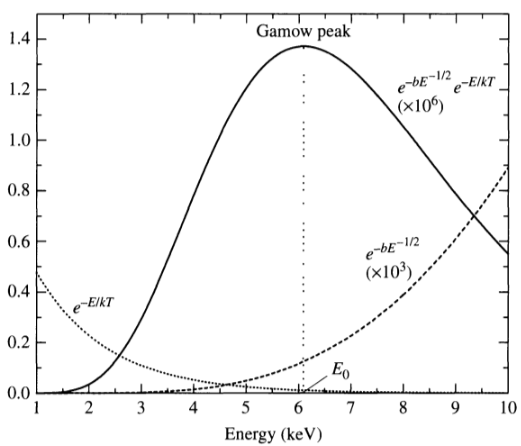
\includegraphics[width=5.6cm]{chapters/10/gamowpeak}
  \caption{核反应可能性示意图。伽莫夫峰是隧穿几率和麦克斯韦-玻尔兹曼速率分布共同作用的结果}
  \label{fig:gamow}
\end{figure}

\newpage
\subsection{核反应类型}
\paragraph{p-p链}
由$^1$H反应生成$^4$He,产能率$\epsilon_{pp}\propto T_6^4$。
\begin{figure}[hbt]
  \centering
  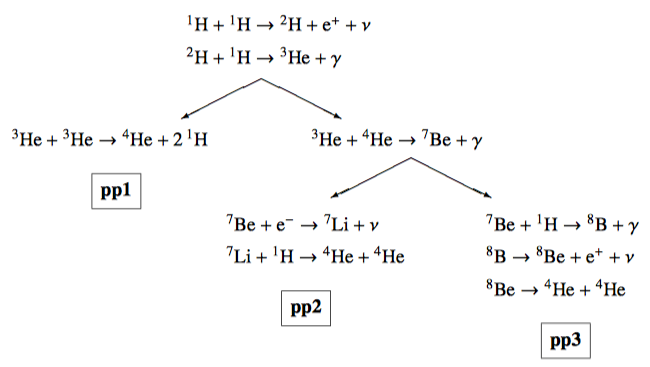
\includegraphics[width=11cm]{chapters/10/ppchains}
  \label{}
\end{figure}


\paragraph{CNO循环}
也是生成$^4$He的核反应,需要温度更高,但是反应更高效,产能率$\epsilon_{CNO}\propto T_6^{19.9}$
\begin{figure}[hbt]
  \centering
  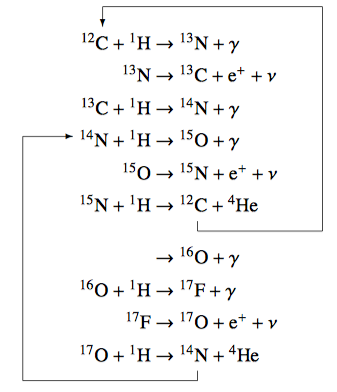
\includegraphics[width=6cm]{chapters/10/cno}
  \label{}
\end{figure}

\paragraph{3$\alpha$反应}
由$^4$He反应生成$^{12}$C,产能率$\epsilon_{3\alpha}\propto T_8^{41}$
\begin{figure}[hbt]
  \centering
  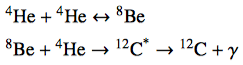
\includegraphics[width=5cm]{chapters/10/3alpha}
  \label{}
\end{figure}



\paragraph{碳氧燃烧}
$^{12}$C和$^{16}$O继续燃烧,生成质量更大的核素\\
\newline
\textcolor{red}{\bf 以上核反应都有各自的点燃温度,温度达到就会开始反应,并且反应速率从上到下关于温度变化越来越敏感}

\begin{figure}[hbt]
  \centering
  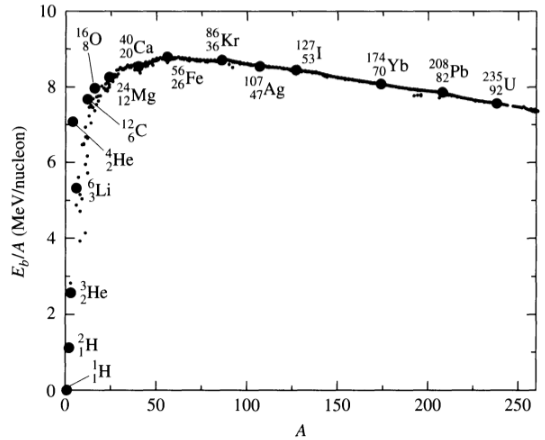
\includegraphics[width=10cm]{chapters/10/bindingenergy}
  \caption{单位核子的结合能。从图中可以看出,铁的位于最大值,铁如果继续聚变生成更重核素就是吸热反应,吸热反应无法在恒星内部自发稳定形成}
  \label{}
\end{figure}



\section{能量转移}
中学时期我们就学过,热传递的三种方式:热传导、热辐射、热对流,能量的传递也是同样的方式
\begin{itemize}
  \item 传导,通过粒子碰撞来传递能量,非常低效,通常在恒星内部不考虑
  \item \textbf{辐射},光子携带能量出去,通过与物质相互作用传递能量
  \item \textbf{对流},通过物质交换形式传递能量,非常高效。但\textbf{产生需满足辐射温度梯度大于绝热温度梯度},即$\nabla_\mathrm{rad}>\nabla_\mathrm{ad}$
\end{itemize}

\paragraph{爱丁顿极限}
当恒星的光度足够大时,光子产生的辐射压在对抗引力的过程中就会占据主导,如果光度继续增加,就会将恒星的物质吹跑,因此这时的光度是恒星能够维持流体静力学平衡的最大光度,称为\textbf{爱丁顿光度},可以通过辐射压与引力平衡计算得到:
\begin{equation}
  L_\mathrm{Ed}={4\pi Gc \over \bar\kappa}M
\end{equation}

\paragraph{沃格特-罗素定理(Vogt-Russel theorem)}
恒星的质量和成分结构就决定了它的半径、光度、内部结构以及未来的演化。

\chapter{太阳}
\section{太阳内部}
\begin{figure}[hbt]
  \centering
  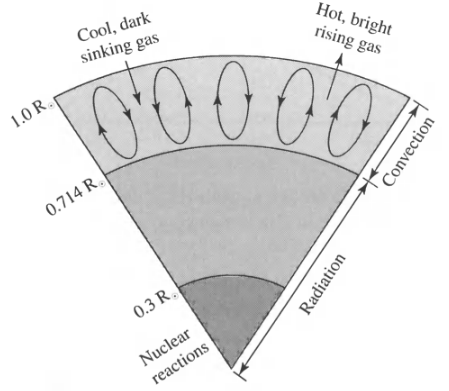
\includegraphics[width=9cm]{chapters/11/interior}
  \caption{太阳内部示意图。太阳内部可大致分为最中心的核反应区、中间的辐射区、最外层的对流区}
  \label{}
\end{figure}

\section{太阳大气}
\begin{figure}[hbt]
  \centering
  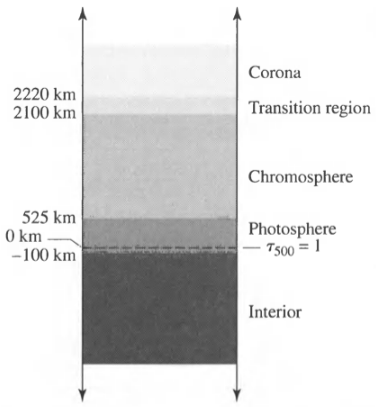
\includegraphics[width=6cm]{chapters/11/atmosphere}
  \caption{太阳大气示意图}
  \label{}
\end{figure}

\subsection{光球层}
光球层是太阳连续谱主要产生的区域,而上方的大气又会在连续谱上产生吸收线,这些吸收线最早由夫琅和费发现,因此被命名为\textbf{夫琅和费线}。

其中$\tau_{500}=1$被定义为\textbf{恒星表面},往下100\,km为光球层底部,往上温度降低,到525km高度降到最低4400\,K,这里被定义为光球层顶部。

观测上能看到恒星表面有明显的被称为\textbf{米粒组织}的对流区域,如图\ref{fig:cell},亮暗是温度不同造成的,亮的区域是高温气体上升到表面,向周围扩散冷却后下沉,对应边缘较暗的区域。

\begin{figure}[hbt]
  \centering
  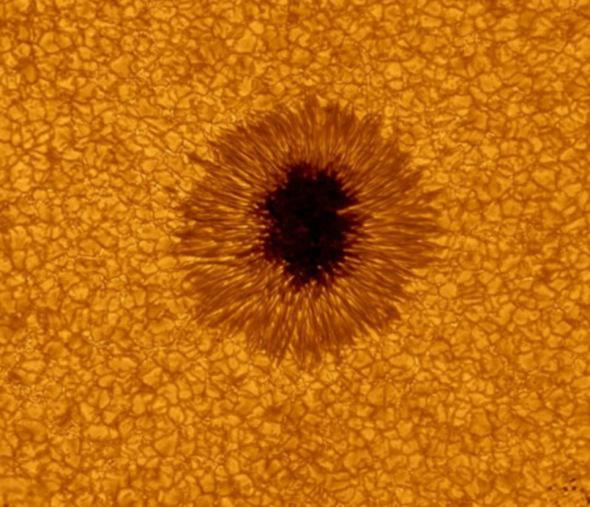
\includegraphics[width=6cm]{chapters/11/cell}
  \caption{米粒组织和太阳黑子}
  \label{fig:cell}
\end{figure}

由于恒星是由气体组成,不像地球这样的固体行星是刚体转动,在任何地方都有相同的自转角速度,恒星在不同纬度和不同深度处的气体自转角速度并不相同,如图\ref{fig:rotaion}所示,太阳维度越高的区域,自转角速度越小,而在内部辐射区以内,极高的密度,使这里的转动接近刚体,具有相同的转速。

\begin{figure}[hbt]
  \centering
  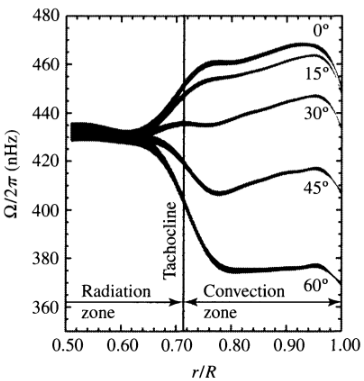
\includegraphics[width=6cm]{chapters/11/rotation}
  \caption{太阳的自选频率随深度和纬度的分布}
  \label{fig:rotaion}
\end{figure}



\subsection{色球层}
光球层之上,太阳表面上方2100\,km以下的范围,是一个很强的谱线产生区域,很多在低温高密度的光球层无法产生的谱线会在这里被产生。

\subsection{过渡区}
位于色球层以上,底部的100\,km,温度从4400\,K上升到$10^5$\,K,变化非常快;后面部分平缓增加到$10^6$\,K,在过渡区的不同高度能够观测到电磁波谱的紫外和极紫外部分。

\subsection{日冕层}
色球层以上,密度和光度都非常低的高温电离区,只有在日食的时候才能够看到日冕,日冕由于密度极低,不适合看作局部热平衡,因此也不适合定义准确温度。观测到的日冕结构可以主要分成以下三部分:
\begin{itemize}
  \item K冕,取自德语的``连续"(\textit{Kontinuierlich}),因为自由电子散射了来自光球层的可见光而被看见
  \item F冕,取自夫琅和费,因为尘埃反射了夫琅和费线而被看见
  \item E冕,由于电离气体的发射线而被看见
\end{itemize}

观测上显示,日冕发出的光并不是均匀的,有的区域比较亮,有的区域比较暗,较暗的区域被称为\textbf{日冕空洞}。这种现象的形成是由于太阳的磁场分布导致的,太阳的磁场近似是偶极磁场,由于磁场线能够束缚等离子体,磁场强的区域会导致比较亮(粒子的辐射)。而在一些磁场``开放''区域,磁场线能够延伸到距离太阳很远的区域,离子也会顺着这样的磁场线逃向远方,这也就形成了\textbf{太阳风}。

高温等离子体中的磁场通常会被``冻结'',从而跟随着等离子体运动,而在在受到一些垂直于磁场方向的扰动时,也会有相应的回复力,同时产生横波——\textbf{阿尔文波}。

\section{太阳周期}
\paragraph{太阳黑子}
如图\ref{fig:cell}黑色部分为太阳黑子,是磁场很强的区域,太阳表面的黑子数量变化会有11年的周期,在此期间,黑子的数量会不断增加,并且向赤道方向靠近。

\paragraph{太阳耀斑}
一种能量释放的过程,其产生机制是由于\textbf{磁重连},相反方向的磁场线靠得较近时,会断裂然后连接形成新的磁场线,在这个过程中会导致原本绕着磁场线旋转的离子被大量抛出。

\paragraph{日珥}
色球层中的一种大型结构,其形成也是与磁场相关

\paragraph{日冕物质抛射}
被认为也是由大型的磁重连事件导致的大量日冕物质被抛出。

\paragraph{太阳磁场}
太阳的磁场近似偶极磁场,同时也具有和太阳黑子一样,每隔11年会倒转N-S极方向,因此目前认为这种现象和太阳黑子的运动有关。由于太阳的较差自转,赤道处的气体比两极快,由于磁冻结效应,赤道处的磁场也会跟着较快自转,这就会导致一段时间后磁场会极度扭曲,发生磁重连。

\chapter{星际介质和恒星形成}
\section{星际尘埃和气体}
恒星和恒星之间实际上存在大量的各种尘埃和气体物质,虽然它们密度很低,但是由于星际间的大尺度距离,它们对星光的散射也是非常可观的。

星际介质对光强的减弱过程被称为\textbf{星际消光},如果将这种影响考虑进对星等的计算,则式\ref{eq:module}变为:
\begin{equation}
  m_\lambda=M_\lambda+5\log_{10}d-5+A_\lambda
\end{equation}

其中$A_\lambda \approx \tau_\lambda$表征星际介质对星等的影响,不同波长的光对应不同的值。

\paragraph{米氏散射理论}
给出任意尺寸的粒子的散射规律。当波长与尘埃直径相近时,散射截面$\sigma_\lambda \propto a^3/\lambda$,$a$为尘埃直径;当波长远小于尘埃直径时,$\sigma_\lambda \propto a^3/\lambda$。简单来说就是\textbf{星际介质对短波长的光散射能力更强},这会导致观测到的光中短波部分会被散射掉,使光看起来偏长波部分,这种现象称为星际红化


\paragraph{中性氢的21\,cm谱线}
如图\ref{fig:21cm},由于质子和电子都有内禀的自旋,两者同向自旋时比反向自旋,电子具有更高的能量,由于低能状态更加稳定,同向自旋的电子最终会变为反向自旋,并辐射出一个光子,这个光子的对应波长为21\,cm。同理,反向自旋的电子也可以吸收一个21\,cm波长的光子激发为反向自旋。

\begin{figure}[hbt]
  \centering
  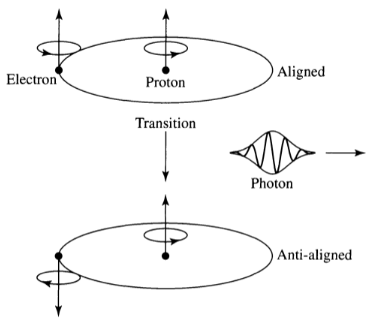
\includegraphics[width=6cm]{chapters/12/21cm}
  \caption{自旋示意图}
  \label{fig:21cm}
\end{figure}

观测上,可以通过21\;cm吸收线来测定中性氢的分布,因为其光深与中性氢柱密度成正比。

\section{原恒星的形成}
星际分子云也是引力束缚系统,前面\ref{virial}节提过稳定的引力束缚系统满足维里定律。反之如果系统的动能和引力不满足维里定理,就不稳定,尤其是当引力势能较大时,分子云就会塌缩。从实际来看,当\textbf{分子云的质量足够大时,一点微小的扰动就会造成分子云的塌缩},这个临界质量称为\textbf{金斯判据}:
\begin{equation}
  M_J\simeq\left({5kT\over G\mu m_H}\right)^{3/2}\left({3\over 4\pi \rho_0}\right)^{1/2}
\end{equation}

\section{主序前的演化}
随着分子云的塌缩,引力势能有一半转换为内能,升高原恒星的温度,还有一半会变成辐射。在塌缩过程中,原恒星在赫罗图\ref{fig:hayashi}上处于最右边近乎垂直的轨迹上,这条轨迹被称为\textbf{林中次郎轨迹},它代表的是流体静力学平衡的分界线,此时原恒星内部会产生大范围的对流来试图改变塌缩产生的温度梯度,达到流体静力学平衡。
\begin{figure}[hbt]
  \centering
  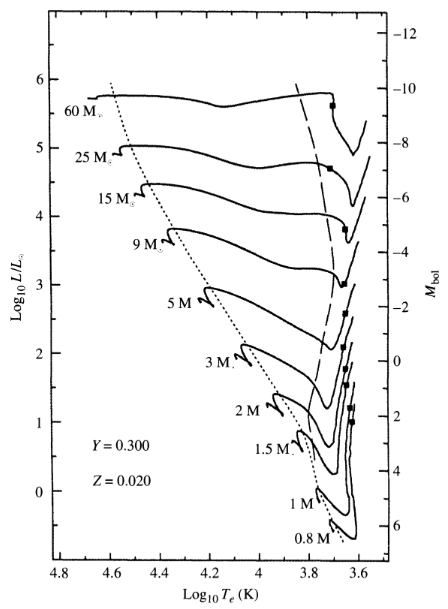
\includegraphics[width=10cm]{chapters/12/hayashi}
  \caption{主序前演化赫罗图}
  \label{fig:hayashi}
\end{figure}

原恒星会持续塌缩,直到温度高到能够平衡引力,而中心的温度是最高的,这时,不同质量的原恒星就会有不同的命运。

质量大于$0.08\,M_\odot$的原恒星在达到平衡前,中心温度会达到氢点燃的温度,开始进行核反应,这时恒星正式进入了主序阶段,该时刻被称为\textbf{零龄主序}。

而对于质量小于$0.08\,M_\odot$的原恒星,它们达到流体静力学平衡时,中心温度不够高,从而只能成为\textbf{褐矮星}。

\begin{figure}[hbt]
  \centering
  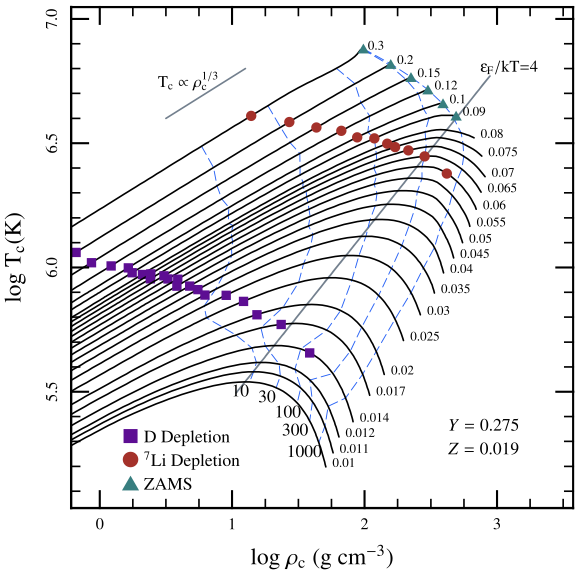
\includegraphics[width=12cm]{chapters/12/prems}
  \caption{不同质量原恒星主序前演化过程中的中心状态图,小于$0.08\,M_\odot$的原恒星无法进入零龄主序。}
  \label{}
\end{figure}

\chapter{主序和主序后的恒星演化}\label{sec:evolution}
\section{不同质量恒星的演化}
\begin{figure}[hbt]
  \centering
  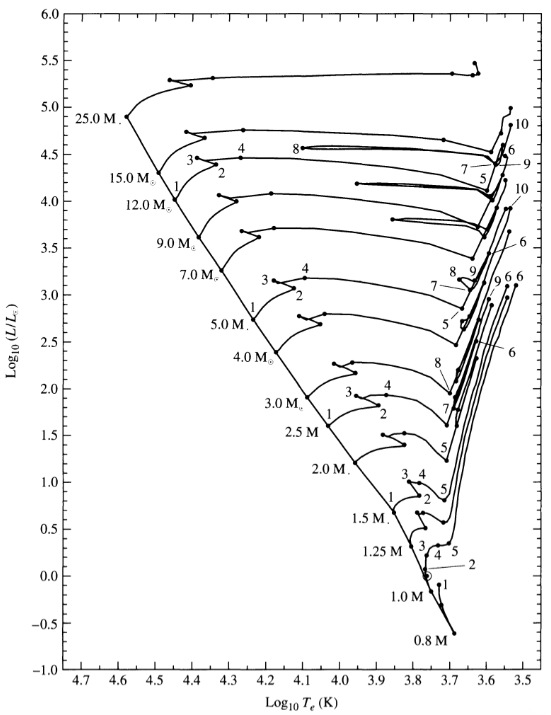
\includegraphics[width=9cm]{chapters/13/HRD}
  \caption{不同质量恒星在赫罗图上的演化}
  \label{fig:HRDM}
\end{figure}

如图\ref{fig:HRDM},不同质量的恒星在进入主序后会有不同的演化命运。可以看到,质量越大的恒星在演化过程中具有更大的温度和光度,在零龄主序处(对角斜线),光度与质量呈幂律分布(因为要满足斯特藩-玻尔兹曼定律)。

对于单个恒星的演化轨迹,一些特征区域需要注意:
\begin{itemize}
  \item 1-3,\textbf{恒星主序演化阶段},主序的定义为中心是氢燃烧阶段。显然发现恒星的主序在赫罗图上并不是简单的一条对角斜线,而是有一定的宽度。
  \item 3-5,\textbf{亚巨星支(SGB)、赫氏空隙},这是中心的氢已经全部核反应完生成了氦核,结束了主序。但是氦核周围还是充满了氢,因此这时会燃烧氦核周围的氢壳层,这会导致恒星会快速膨胀,到达最右侧的林中次郎轨迹。这时恒星的对流区域能够达到很深的范围,会将外部物质与内部物质混合交换,被称为\textbf{第一次挖掘}。之所以称为空隙是因为恒星在这个阶段演化非常快,观测上很少能够观测到这个阶段的恒星,因此在赫罗图上形成了一段空白区域。
  \item 5-6,\textbf{红巨星支(RGB)},因为恒星膨胀到一定程度会达到平衡极限,因此之后会沿着林中次郎轨迹演化。氢壳层燃烧生成氦,增加氦核的质量,并提高氦核的温度。
  \item 6-9,\textbf{氦核燃烧},通过3$\alpha$反应生成$^{12}$C。
  \item 9-10,\textbf{渐进巨星支(AGB)},氦核完全变成碳核,周围的氦壳层燃烧,恒星再次膨胀,并在此经历\textbf{第二次和第三次挖掘}。
\end{itemize}


\begin{figure}[hbt]
  \centering
  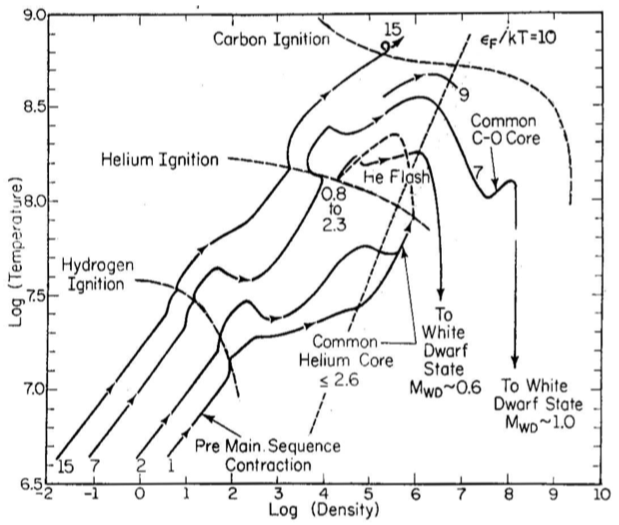
\includegraphics[width=10cm]{chapters/13/center}
  \caption{不同质量恒星中心的状态演化}
  \label{fig:center}
\end{figure}

如图\ref{fig:center},不同质量恒星在演化过程中,核心也经历了不同的命运。刚开始它们都经历了原恒星的塌缩阶段,直到中心的氢点燃,之后的演化会开始出现分歧。

$1\,M_\odot$和$2\,M_\odot$的恒星由于反应是温度和质量不够,会形成简并的氦核,然后通过氢壳层燃烧缓慢增长氦核的质量,直到氦核达到点燃温度,首先会解除氦核的简并,这一步称为\textbf{氦闪},然后稳定燃烧。

而$7\,M_\odot$和$15\,M_\odot$的恒星因为质量比较大,中心的温度会更高,在形成氦核之后温度自然达到点燃温度直接进行氦核燃烧,没有了简并的过程。这时大家都在进行氦核燃烧生成碳-氧核的过程,然后又会发生分歧。

$1\,M_\odot$、$2\,M_\odot$和$7\,M_\odot$的恒星在形成碳-氧核之后,温度不够点燃,又会发生简并,不幸的是,现在就算氦壳层的燃烧也不足以把碳-氧核的温度提高到点燃温度,它们会形成一般的\textbf{碳-氧白矮星}。

而$15\,M_\odot$的恒星能够有效的直接发生碳-氧核,甚至不发生简并阶段。

根据以上的演化过程,我们可以将恒星进行分类
\begin{itemize}
  \item 以氦核是否发生简并为界,区分小质量恒星和中等质量恒星,一般界限为$2\,M_\odot$
  \item 以碳-氧核是否发生简并为界,区分中等质量恒星和大质量恒星,一般界限为$8\,M_\odot-11\,M_\odot$
\end{itemize}

\begin{figure}[hbt]
  \centering
  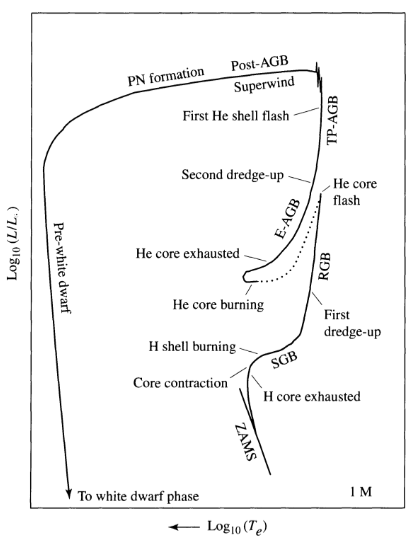
\includegraphics[width=6.4cm]{chapters/13/lowmass}
  \caption{小质量恒星的演化轨迹}
  \label{}
\end{figure}

\begin{figure}[hbt]
  \centering
  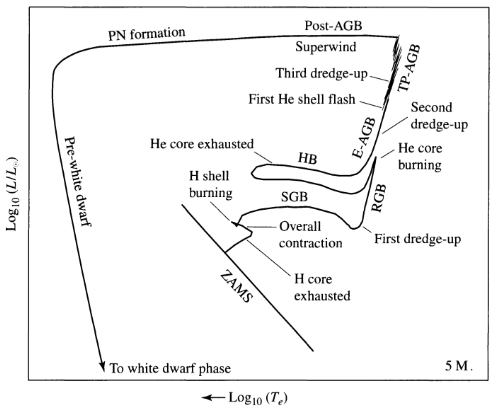
\includegraphics[width=8cm]{chapters/13/intermediate}
  \caption{中等质量恒星的演化轨迹}
  \label{}
\end{figure}

当恒星演化到渐进巨星支时,半径很大会导致表面引力束缚变弱,星风活动就会变得剧烈,引起恒星的质量损失。恒星演化到渐进巨星支后期时甚至会产生超星风,这类恒星因为在红外波段的光度最强,且能探测到羟基分子,被称为红外羟基源(OH/IR sources)。羟基分子的探测是通过羟基产生的\textbf{脉泽}实现的。脉泽即微波波段的激光,受到激发的电子从基态跃迁到第一激发态,后又退激发。但没有回到基态,而是集中在了亚稳态,当处与亚稳态的粒子集体跃迁到基态时,就产生了能量较大的微波。


\section{星团}
\subsection{星族}
恒星诞生于分子云,以星际介质为原料,而金属元素通常由恒星的核反应生成,因此恒星的分类不仅可以按照质量划分,还可以根据金属丰度来划分:
\begin{itemize}
  \item 星族III,或者第一代恒星,不含金属元素,诞生于宇宙最早期,当时的原料只有氢氦
  \item 星族II,金属丰度很低,原料基于部分第一代恒星产生的金属
  \item 星族I,金属丰度较高,最年轻的一代
\end{itemize}

\subsection{球状星团和疏散星团}
如果分子云较大,在塌缩的过程中会碎裂,分别形成恒星,这样就形成了星团。
\paragraph{球状星团}
恒星数量很多,年龄较大,分布较密集。
\paragraph{疏散星团}
恒星数量比较少,年龄较小,分布比较稀疏。

由于恒星的演化速率和质量呈正相关,质量越大,恒星的演化速度越快,因此可以通过如图\ref{fig:cluster}星团内恒星的演化来分析星团的年龄。
\begin{figure}[hbt]
  \centering
  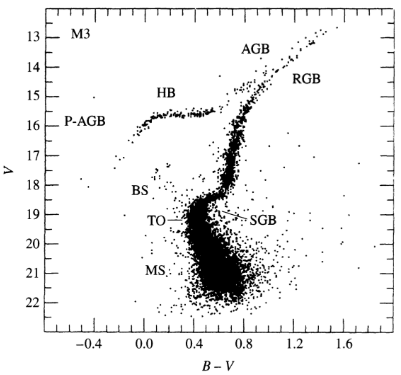
\includegraphics[width=6cm]{chapters/13/cluster}
  \caption{星团的颜色-星等图,等价于赫罗图。由于星团内恒星几乎同时诞生,质量越大,越早离开主序阶段,可以根据主序带上的拐点来确定星团的年龄。}
  \label{fig:cluster}
\end{figure}

\paragraph{赫氏空隙}
人们在一些星团的颜色-星等图中发现,主序阶段和红巨星阶段的恒星分布之间并不连续,两者之间的恒星分布很少,在图中形成了较空白的区域,这被称为赫氏空隙。赫氏空隙的产生是由于恒星在亚巨星支上的演化是热力学时标,很快就过去了,于是留下个空隙。

\chapter{恒星脉动}
\section{脉动星}
由于恒星在演化过程中会发生膨胀和收缩,这些都是恒星内部维持平衡而产生的过程,这些膨胀和收缩导致的是恒星气体发生运动,形成一种类似驻波的周期性脉动,使恒星的半径发生周期性变化,进而导致光度发生周期性变化。

形象来看,这种波动在恒星内部以声速$v_s=\sqrt{\gamma P/\rho}$来回传播,可以想象,对于半径越大的恒星,其光度越强,波动传播时间越长,脉动周期就越长,这种\textbf{脉动恒星的周光关系}最早被哈佛大学的列维特所发现,计算也可以得到周期和密度的关系:
\begin{equation}
  \Pi\approx\sqrt{3\pi \over 2\gamma G\rho}
\end{equation}

\begin{figure}[hbt]
  \centering
  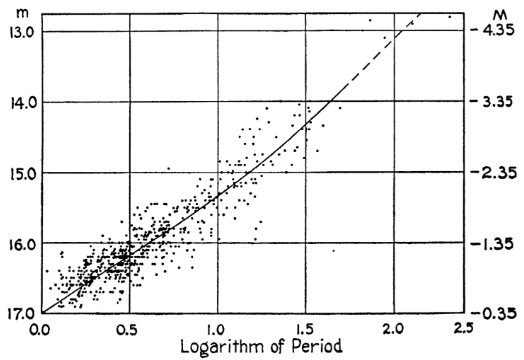
\includegraphics[width=8cm]{chapters/14/cepheid}
  \caption{经典造父变星的周光关系}
  \label{}
\end{figure}

恒星的膨胀和收缩是为了平衡引力,因此正常情况下恒星能够通过这种方式会恢复平衡,而不会演化成周期性的脉动,但是如果有些特殊机制,阻碍其有效平衡引力,就会维持这种膨胀和收缩,形成脉动。

在恒星的绝大部分区域,压缩会使温度升高,不透明度下降;而在\textbf{部分电离区},压缩时一部分压缩功会用于电离,令粒子数密度增加,不透明度反而上升。这会令从内部传播出来的光子无法有效通过,能量会在这里积累,温度上升,又会导致膨胀;同样,膨胀时温度降低,不透明度降低,同时离子结合放出的光子很容易逃离,带走能量,又回导致压缩,形成新的循环。这种不透明度导致脉动的机制被称为\textbf{$\kappa$机制}。

同时,因为部分电离区的压缩会引起电离,因此这里的温度上升程度比周围小,会引起周围的热量向这边传递,这会增强$\kappa$机制,而这种效应被称为\textbf{$\gamma$机制}。

部分电离区在脉动中的作用就像一个弹簧,在恒星膨胀和收缩过程中通过电离和结合的形式吸收和释放能量,维持住脉动。

脉动星在脉动时,会有不同的波动模式,有径向波动和非径向的波动,根据波动模式不同可以将脉动星分为不同类别,并在赫罗图中有对应的不同\textbf{脉动带}区域,当恒星演化到相应区域时会产生相应的脉动,如图\ref{fig:pusating}。

而有些人认为脉动带远不止这些,而我们的太阳就处于一种一条内,由于脉动周期在3-8分钟之间,因此被称为\textbf{五分钟振荡}。

\begin{figure}[hbt]
  \centering
  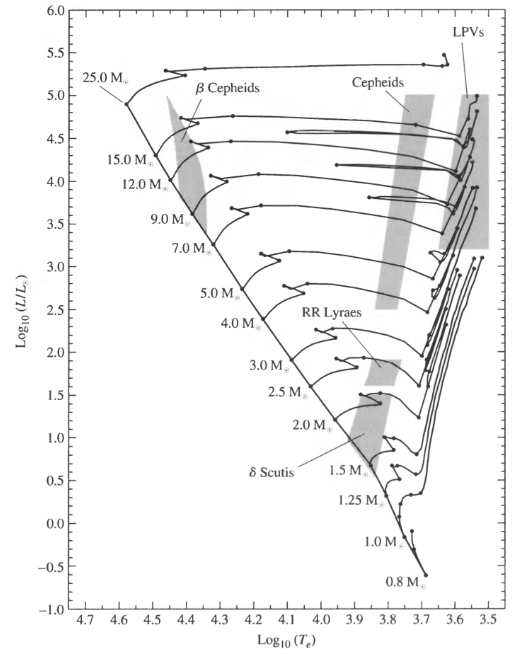
\includegraphics[width=10cm]{chapters/14/pusating}
  \caption{赫罗图上的脉动带}
  \label{fig:pusating}
\end{figure}

\chapter{大质量恒星的命运}
\section{大质量恒星的主序后演化}
前面提到大质量恒星的演化相较中等质量和小质量恒星要顺利的多,每一步点燃温度都能直接达到,随后进行一步步的核反应,最终能生成铁核。

同时也因为温度高,大质量恒星的核反应速率非常快,演化速率也非常快,并且伴随着剧烈的星风,和较大的质量损失率。

\begin{figure}[hbt]
  \centering
  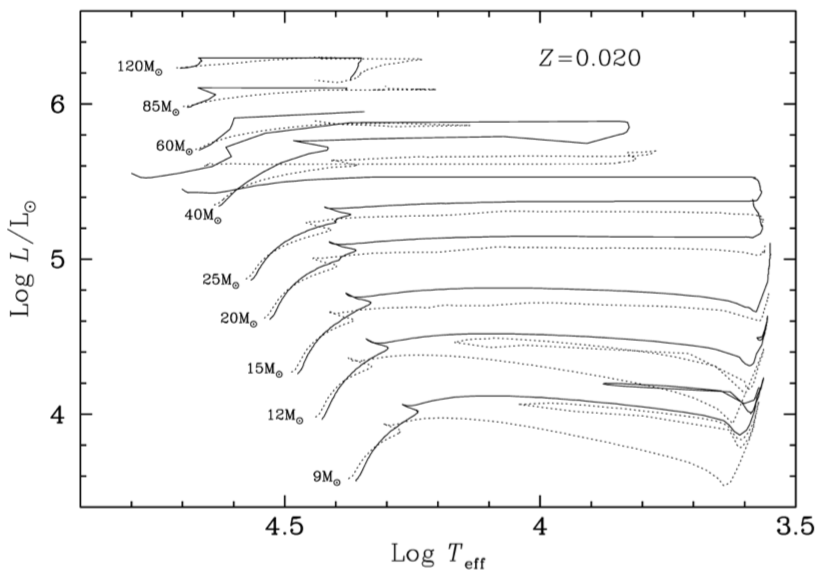
\includegraphics[width=10cm]{chapters/15/massive}
  \caption{大质量恒星的演化轨迹。实线考虑自转,虚线不考虑自转。}
  \label{}
\end{figure}

\section{超新星}
铁核形成后,因为铁的核反应过程是一个吸热过程,因此恒星无法继续平衡,最终导致恒星塌缩,然后发生超新星爆发。超新星爆发会抛离恒星的外层物质,留下中心的简并核,根据核的质量不同,分别会形成白矮星、中子星和黑洞。

在超新星爆发过程中,比铁更重的元素会被生成。宇宙中的超新星爆发来源并不是只有大质量恒星的塌缩,不同的来源会导致它的光谱也不同,因此人们根据以下几个原则对超新星进行分类,详细分类见图\ref{fig:supernova}:
\begin{itemize}
  \item 有无氢线,无氢线的超新星由于最早被发现,被定义为I型超新星,有氢线为II型超新星
  \item 有无硅线,I型超新星中有硅线的为Ia型,无硅线为Ib和Ic
\end{itemize}

\begin{figure}[hbt]
  \centering
  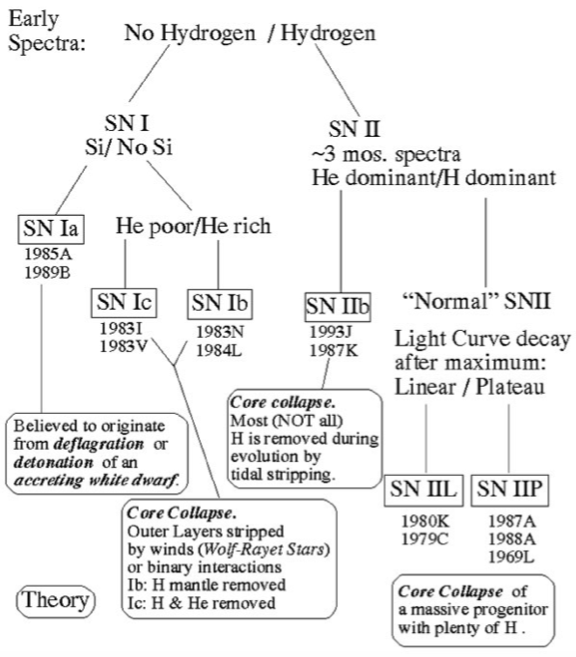
\includegraphics[width=10cm]{chapters/15/supernova}
  \caption{超新星的详细分类}
  \label{fig:supernova}
\end{figure}

\section{伽马射线暴}
上世纪美苏冷战期间,为了监视苏联的核试验,美国发射了卫星来探测苏联的伽马射线源,却因此意外地发现了\textbf{伽马射线暴}现象。通过对伽马射线暴的长时间检测,人们发现它们在天空中的分布几乎是均匀的,因此确定它们的来源主要是\textbf{银河系以外}。

伽马射线暴主要表现为天空中某个方向的伽马射线强度突然出现短暂峰值,当天文学家把观测到的伽马射线线按照持续时间分类后发现,它们以2\,s为界明显分为两类——\textbf{长暴和短暴},其中短暴能量高,长暴能量低。

\chapter{恒星的简并残骸}
上章讲到,大质量恒星超新星爆发后,会抛离周围大部分物质,中心留下简并核,根据核的质量不同会形成白矮星、中子星或黑洞等致密星。

\section{白矮星}
白矮星内部主要由电子简并压抵抗引力,其质量和太阳相当,但大小和地球差不多。白矮星内部没有核反应进行,表面温度5,000\,K到80,000\,K不等,同样我们根据白矮星的光谱可以将其分为五类:
\begin{itemize}
  \item DA,占总数的三分之二,有碰撞增宽的氢吸收线
  \item DB,占总数的$8\%$,只有氦吸收线
  \item DC,占总数的$14\%$,没有谱线的连续谱
  \item DQ,光谱中含碳线
  \item DZ,光谱中有金属线
\end{itemize}

\paragraph{白矮星冷却时标}
白矮星的电子由于简并,导致低能级占满,无法从更高能级下来,因此白矮星辐射的热量主要来自原子核的动能。因此假设白矮星质量为$M_\mathrm{wd}$,原子质量为$Am_H$,就可以得到原子数,因为每个原子核的内能是${2\over 3}kT$,就可以计算出总内能,配合白矮星的光度,可以得到
\begin{equation}
  \tau_\mathrm{cool}={U\over L_\mathrm{wd}}={3\over 2}{M_\mathrm{wd}k\over Am_H C T_c^{5/2}}
\end{equation}

代入典型值可以得到$\tau_\mathrm{cool}\approx 170$\;百万年,从式中还可知温度越低白矮星冷却的越慢,因此白矮星大部分时候以较低的温度和光度缓慢冷却。

\subsection{简并}
根据泡利不相容原理,不能有两个费米子具有相同的量子态,而能级的量子态总数是有限的。因此当物质的密度很大时,会产生简并压,以防止更多的粒子被压至相同的轨道。那么简并压是否有上限?

由于费米子除了遵循泡利不相容原理,还要符合海森堡不确定性原理,因此当电子被压得相互之间很靠近时,其位置不确定性会减小,动量的不确定性会增加,速度也因此增加,而速度的最大不能超过光速,这就是简并压的上线。

1931年,印度物理学家钱德拉塞卡由此计算了电子简并压的上限,并提出了白矮星的质量上限——\textbf{钱德拉塞卡极限}$M_\mathrm{Ch}=1.44\,M_\odot$。

\section{中子星}
那么当白矮星的质量超过钱德拉塞卡极限之后会怎么样?电子会被压缩进原子核,与质子合并形成中子,中子星就由此诞生了。

一颗质量与太阳相当的中子星,直径大约只有10\,km。中子星内部由中子简并压抵抗引力,由于中子具有比电子更大的质量,因此它的简并压上线比电子大得多。同时由于体积的压缩,为了满足磁通量守恒,中子星的磁场非常强$B\sim10^{12}\,$G。

\section{脉冲星}
脉冲星是一类特殊的天体,观测上表现为周期性的脉冲信号,并且周期很短,最低达到毫秒量级,最高在秒量级。

目前大家公认为是脉冲星本质是中子星,如图\ref{fig:pulsar},中子星的磁场也是偶极磁场,被磁场捕获的带电粒子在沿两极被抛出,这就是脉冲的来源。而在白矮星塌缩至中子星的过程中,也要满足角动量守恒,因此中子星的自转周期非常短,这也解释了脉冲星短周期的原因。

\begin{figure}[hbt]
  \centering
  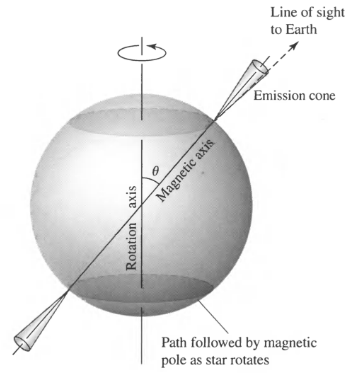
\includegraphics[width=8cm]{chapters/16/pulsar}
  \caption{基本的脉冲星模型}
  \label{fig:pulsar}
\end{figure}

由于脉冲星周围的强磁场,当捕获带电粒子之后,带电粒子绕旋磁场线运动,会产生辐射。如果捕获的是相对论性(速度接近光速)带电粒子,会产生\textbf{同步辐射};如果磁场很强,或带电粒子的入射角很小,导致回旋半径很小,那么带电粒子就好像是沿着磁场线运动一样,这时产生的是\textbf{曲率辐射}。

脉冲星中还有一类特殊的群体——\textbf{软伽马射线复现源},这类被认为是由具有更强磁场的中子星——\textbf{磁星}所产生的

\paragraph{光速圆柱面(光柱面)}
带电粒子被中子星磁场捕获后,会随着磁场与中子星同步转动,但在距离中子星自转轴$R_c=c/\omega=cP/2\pi$处,如图\ref{fig:lightcylinder},同步速度达到光速,带电粒子无法继续没束缚,就会被甩出去,并产生同步辐射或曲率辐射。

\begin{figure}[hbt]
  \centering
  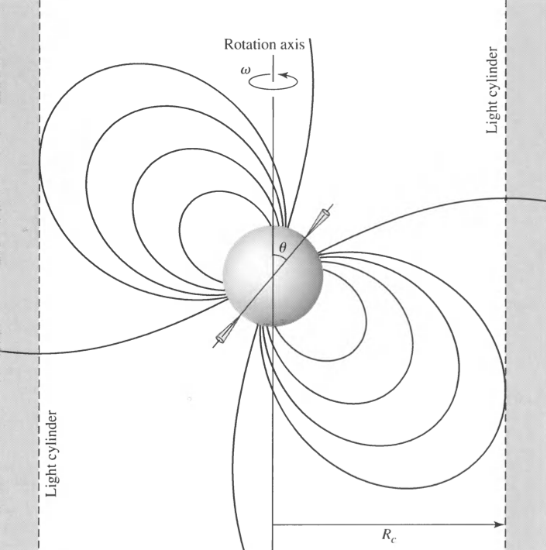
\includegraphics[width=10cm]{chapters/16/lightcylinder}
  \caption{中子星周围的\textbf{光柱面}。}
  \label{fig:lightcylinder}
\end{figure}

\setcounter{chapter}{17}
\chapter{密近双星}
\section{密近双星系统的引力}
如图\ref{fig:binary}所示,在双星系统中,引力等势面呈现为``8''字型,这个等势面被称为\textbf{洛希瓣},中间的交点为引力平衡点,被称为\textbf{拉格朗日点}。

\begin{figure}[hbt]
  \centering
  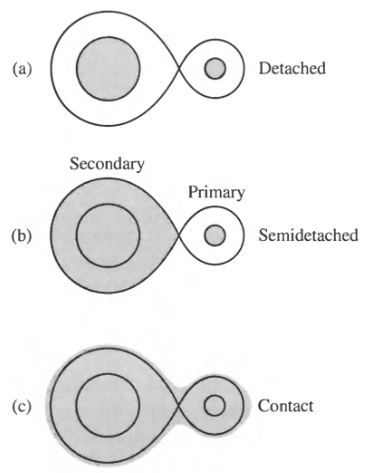
\includegraphics[width=6cm]{chapters/18/binary}
  \caption{双星系统的分类}
  \label{fig:binary}
\end{figure}

当两颗星距离足够远时,它们之间几乎不发生相互作用,属于\textbf{分离}形双星系统。

当两颗星足够近,且一颗恒星膨胀至洛希瓣时,由于引力的作用其性质也会变成泪滴状,并且拉格朗日点附近的物质一旦越过拉格朗日点,就会受另一颗星的引力作用而被吸引过去,这种属于\textbf{半分离}形双星系统。其中接受物质的恒星被称为\textbf{主星},失去物质的被称为\textbf{次星}。

如果两颗双星都充满了洛希瓣,那么它们之间就可以很容易地发生物质交换,这种属于\textbf{相接}形双星系统。

通过计算可以得到拉格朗日点当两星重点的距离分别为:
\begin{align}
  \ell_1 &=a\left[0.500-0.227\log_{10}\left({M_2\over M_1}\right)\right]\\[2mm]
  \ell_2 &=a\left[0.500+0.227\log_{10}\left({M_2\over M_1}\right)\right]
\end{align}

其中下标1代表主星,下标2代表次星。

\section{吸积}
对于半分离形双星系统,主星吸引次星越过拉格朗日点的物质的过程被称为\textbf{吸积},并会在周围形成\textbf{吸积盘},假设双星模型为两个交叠的圆,单位时间吸积质量的多少用\textbf{质量转移率(吸积率)}来描述:
\begin{equation}
  \dot M\approx \pi Rd\rho \sqrt{3kT\over m_H}
\end{equation}

其中$R$为洛希瓣半径,$d$为交叠的长度。

\section{双星系统的演化}
首先考虑两颗星初始是分离型双星系统,当一颗较小质量恒星演化为红巨星膨胀时,会填充洛希瓣,变成半分离形双星系统。随着主星的吸积,次星的质量会减小,引力会减弱,洛希瓣因此收缩,这会进一步增加吸积率,加快主星的吸积。

之后双星系统会被次星的物质所包围,变成相接双星系统,次星只剩下了简并核。双星在气体团中运动时会与气体摩擦,损失角动量,轨道会缩小,这可能会导致两颗星的并合,形成单星。

如果双星没有并合,反过来,轨道缩小也会导致洛希瓣缩小,原来的主星填满了洛希瓣,继而变成了次星,被反向吸积,但是因为现在的次星有较大的质量,吸积率会被维持在一个稳定的速率,最终变成两个轨道近密的双白矮星。其中一个质量较小、体积较大的白矮星会超出它的洛希瓣,然后分解在另一颗质量较大的白矮星周围形成吸积盘,如果主星吸积之后质量超过钱德拉塞卡极限,则会产生Ia型超新星爆发。

以上演化过程见图\ref{fig:binaryevolution},需要注意的是这只是一种设想,实际演化过程会受多种因素影响。

相接双星系统也可以分成多种种类,而很多是根据最早发现的相应的天体命名的:
\begin{itemize}
  \item 大陵五,两个一般恒星组成的半分离系统
  \item 猎犬座RS和天龙座BY,色球层活跃双星
  \item 大熊座W型相接双星,磁场活跃度很高
  \item 激变变星和类新星双星,白矮星和冷的M形次星
  \item 黑洞和中子星组成的X射线双星
  \item 御夫座ζ和仙王座VV,晚型超巨星和热的(一般为B星)伴星
  \item 共生双星,M型巨星被白矮星、亚矮星或低质量主序星吸积
  \item 钡和S光谱型星,白矮星和S光谱型(K型和M型之间)次星
  \item 共包层后双星,热白矮星和较冷次星
\end{itemize}

\begin{figure}[hbt]
  \centering
  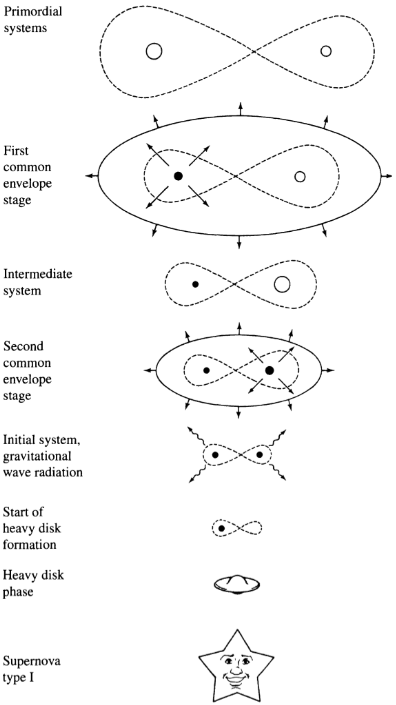
\includegraphics[width=9cm]{chapters/18/evolution}
  \caption{双星系统演化示意图}
  \label{fig:binaryevolution}
\end{figure}

\section{Ia型超新星}
前面描述到,主星白矮星在吸积次星白矮星分解后的物质,当质量达到钱德拉塞卡极限时,会产生Ia型超新星爆发,这是\textbf{超新星的一种产生模型}。\textbf{另一种模型}也可以是白矮星吸积正常恒星的物质,达到钱德拉塞卡极限后也会产生Ia型超新星。而这两种模型中,物质落在白矮星上产生超新星,会将白矮星也炸毁。

由于爆发时质量都为$1.4\,M_\odot$,爆发时的光度也就基本都相同,因此Ia型超新星可以作为标准烛光来测定距离。

\paragraph{毫秒脉冲星}
被认为产生于X射线双星中,但依旧可以分为两类:在大质量X射线双星中的毫秒脉冲星具有大质量的伴星(中子星),这类公转周期短且为偏心轨道;低质量X射线双星中的具有低质量伴星(白矮星),这类公转周期长且为圆轨道


\part{The Solar System}
\chapter{太阳系中的物理过程}
\section{潮汐力}
如图\ref{fig:tidalforce} 由于地球本身尺度的原因,导致地球表面收到的月球引力不相等,产生差引力,这被称为\textbf{潮汐力}。地球上近月球端和远月端的潮汐力方向相反,这会使地球发生延地月连线方向的形变,引起涨潮现象,因此这种形变被称为\textbf{潮汐隆起}。

\begin{figure}[hbt]
  \centering
  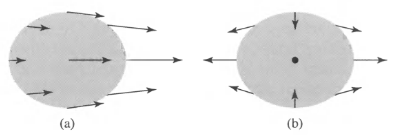
\includegraphics[width=10cm]{chapters/19/tidalforce}
  \caption{潮汐力示意图。(a)地球表面月球的引力(b)月球对地球的潮汐力(表面与地心的差引力)}
  \label{fig:tidalforce}
\end{figure}

为了理解潮汐力和潮汐隆起,尤其是背面的潮汐隆起,我们需要明白地球上每一点都受到月球的引力,近月段最强,中心较弱,远月端最弱。因此近月端的海水被拉像月球产生潮汐隆起,而远月端因为落后于被月球拉走的地球而产生隆起。两端的潮汐隆起导致了我们一天能看到两次涨潮。

通过计算,我们可以得到引力随距离的大小变化为:
\begin{equation}
  dF_m=-2G{Mm\over r^3}\;dr
\end{equation}

对于地球来说,可以得到潮汐力为:
\begin{equation}
  \Delta F\simeq{GMmR\over r^3}\left(2\cos\theta\,\hat{\mathbf i}-\sin\theta\,\hat{\mathbf j}\right)
\end{equation}

其中$R$是地球半径,$r$是地球中心到月球的距离,$\theta$是地球表面一点与地月方向的夹角,而在地月连线上$\Delta F=-2G{Mm\over r^2}$。从式中可以发现,两个天体距离越近的时候,潮汐力越显著。

\begin{figure}[hbt]
  \centering
  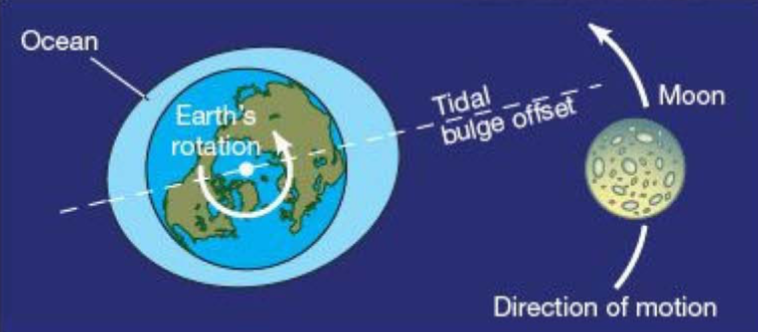
\includegraphics[width=10cm]{chapters/19/tidalbulge}
  \caption{地球自转引起潮汐隆起不准确指向月球}
  \label{fig:tidalbulge}
\end{figure}

潮汐力的另一个作用是会使地球的自转变慢。如图\ref{fig:tidalbulge},由于地球的自转比公转快,地壳与海洋以及地球内部的摩擦效应会使潮汐隆起会有被拖动着与地球一起转的趋势,这导致了隆起部分并不严格指向月球,而这种长期的摩擦会导致地球的自转变慢,最终与公转周期相同,这种效应被称为\textbf{潮汐锁定}。月球就是一个已经被地球的潮汐力锁定的天体,因此月球永远是固定的一面朝着我们。

\subsection{洛希极限}
那么我们可以想象,当潮汐力足够大的时候,天体甚至能够被撕裂,这种现象常常发生在黑洞这类的致密星附近。要撕裂一个天体,潮汐力需要克服引力,前面算出,距离越近,潮汐力越强,洛希在1850年计算得到了这个临界距离,此后被称为\textbf{洛希极限}:
\begin{equation}
  r<f_R\left(\bar \rho_P \over \bar \rho m\right)^{1/3}R_p
\end{equation}

其中$f_R=2.456$。

\section{大气的物理}
\subsection{大气温度}
行星的温度来源于太阳的辐射,因此我们可以考虑行星的反照率为$a$,即吸收了(1-$a$)倍的辐射升温,同时行星还会以黑体辐射的方式辐射热量,假设到太阳的距离为$D$,我们可以计算出热平衡下行星大气的温度为:
\begin{equation}
  T_p=T_\odot(1-a)^{1/4}\sqrt{R_\odot \over 2D}
\end{equation}

\subsection{大气成分}
由于行星的大气之外是真空,时刻在做无规则热运动的气体分子受行星引力束缚在行星表面,但温度越高,气体分子运动越剧烈,就越有可能逃离行星。

根据麦克斯韦-玻尔兹曼速率分布和行星表面的逃逸速度,我们可以计算得到分子的逃逸温度:
\begin{equation}
  T_\mathrm{esc}>{1\over54}{GM_p m \over kR_p}
\end{equation}

其中$m$是气体粒子的质量。通过上式可以知道,质量越大的粒子可以在较高温度的大气中存在,较轻的粒子则会逃离行星表面。结合前面计算得到的行星大气温度,我们可以知道行星大气中可能存在的气体成分。

\setcounter{chapter}{21}
\chapter{太阳系的小天体}
\section{彗星和柯伊伯带天体}
\paragraph{彗星}
主要成分为水冰,含少量一氧化碳冰、二氧化碳冰以及尘埃,因此彗星模型又被称为脏雪球模型。具有很大的轨道偏心率,根据周期长度可以分为以下两类:
\begin{itemize}
  \item \textbf{短周期彗星},公转周期短于200年,轨道靠近黄道面,频繁进入内太阳系,来源于柯伊伯带,哈雷彗星就是典型的短周期彗星
  \item \textbf{长周期彗星},公转周期长于200年,轨道不在黄道面上,奥尔特云
\end{itemize}

\paragraph{奥尔特云}
位于太阳系的最外围,距离太阳3,000\,AU到100,000\,AU的区域,包含了大约$10^{12}-10^{13}$个、质量约为$100\,M_\odot$的成员。奥尔特云内区(3,000\,AU到20,000\,AU)主要集中在黄道面上,外区(20,000\,AU到100,000\,AU)以球形包裹着太阳系。

\paragraph{柯伊伯带}
位于海王星以外,距离太阳30\,AU到50\,AU的区域,是位于黄道面内包含大量彗核的盘。冥王星是第一颗被发现的\textbf{伊伯带天体}。

\section{小行星}
太阳系内大部分小行星位于火星和木星轨道之间的小行星带内,是没有形成行星的星子。

小行星带中的小行星大小不等,最大的三颗小行星分别是智神星、婚神星和灶神星,平均直径超过400\,km;仅有的一颗矮行星—谷神星,直径约为950\,km。

小行星带中有一条密度较低的区域被称为柯克伍德空隙,是由于3:1的轨道共振所产生的。

\paragraph{特洛伊小行星}
还有一部分小行星位于木星轨道,与木星和太阳成等边三角形的区域。由于该区域是木星和太阳的拉格朗日点$L_3$和$L_4$,是引力势能最低点,因此小行星能够稳定在这里绕太阳公转。

\chapter{行星系统的形成}
前面讲到恒星是通过分子云塌缩形成的,但是如果分子云在一开始具有角动量(很普遍),那么在塌缩过程会形成一个吸积盘。

吸积盘会导致最终只有核心部分会形成恒星,而周围的物质会形成\textbf{残骸盘}。而在残骸盘冷却的过程中,一些尘埃颗粒会吸附周围的物质,形成质量越来越大的球,表面积也越大,越容易碰撞和吸附到新物质。

当球的质量大到可以用引力吸引周围物质时,便成为了\textbf{星子},星子体积与小行星大小相当。然后星子会进一步清扫轨道内和附近的物质,形成较大的天体,最终形成行星。

为了描述星子清扫周围物质的能力,我们可以假设如果微粒绕星子公转的周期等于星子绕太阳公转的周期,那么微粒就会被星子引力束缚,这时的半径被称为\textbf{希尔半径}:
\begin{equation}
  R_H=\left({M\over M_\odot}\right)^{1/3}a=\left({R\over R_\odot}\right)\left({\rho \over \rho_\odot}\right)^{-1/3}a={R\over \alpha}
\end{equation}

其中$a$是星子的轨道半长轴,$R$是微粒到星子的距离,计算时可认为是星子的大小。

\part{Galaxies and the Universe}
\chapter{银河系}
\section{银河系的形态}
千亿颗恒星构成了银河系,太阳到银河系中的距离约为8\,kpc,银河系的结构整体呈现为漩涡状,其中大致可分为一下几部分:
\begin{itemize}
  \item 银盘,恒星主要分布的区域,直径约为50\,kpc。根据成分不同可以分为薄盘和厚盘:薄盘包含较年轻的恒星和星际介质,垂直标高为350\,pc;厚盘包含年龄较大的恒星,银道面上的恒星密度只有薄盘的8.5\%,垂直标高可达1000\,pc
  \item 银核,银河系中心恒星密度很大,光度很大的区域,半径可达0.7\,kpc
  \item 银棒,位于银河系中心,半径可达4\,kpc
  \item 银晕,银盘周围的球形气体,半径可达100\,kpc,其中分布着星团
  \item 暗物质晕,整个银河系都镶嵌在暗物质晕中,半径可达230\,kpc,具有银河系的极大部分质量
\end{itemize}

由于金属元素只能通过核反应合成,而铁元素主要通过超新星爆发产生,因为中小质量很无法生成合成铁,而大质量恒星只能生成铁核,核的质量毕竟很少。根据这种性质,我们可以认为恒星在演化过程中几乎不生成铁,那么类似前面的星族分类,年轻的恒星往往铁含量较高,因为是基于前代恒星的残骸形成,而年老的恒星形成很早,铁含量很低,类比到金属含量也是相同的规律,这种规律被称为\textbf{年龄-金属丰度关系}。由此我们可以通过铁来定义\textbf{金属丰度},且和恒星年龄有相关性:
\begin{equation}
  [\mathrm{Fe/H}]\equiv \log_{10}\left[{(N_\mathrm{Fe}/N_\mathrm{H})_\mathrm{star}\over (N_\mathrm{Fe}/N_\mathrm{H})_\odot}\right]
\end{equation}

上式以太阳为基准来定义金属丰度,因此太阳的$[\mathrm{Fe/H}]=0.0$。

根据引力的作用效果,考虑暗物质晕的密度分布应遵循
\begin{equation}
  \rho(r)={\rho_0 \over (r/a)(1+r/a)^2}
\end{equation}

在远离银晕的区域密度以$1/r^2$减小分布,在靠近中心处稍微平缓一点以$1/r$分布。

\section{银河系中心}
银河系的中心位于半人马座A的方向,从那个方向还能观测到X射线,其来源被认为就是银河系中心。其产生原因目前普遍认为是\textbf{银河中心存在着一个超大质量黑洞},质量$\sim 4\times 10^6\,M_\odot$。

\chapter{星系的性质}
\section{星系分类}
目前最广泛使用的星系分类是\textbf{哈勃序列}。哈勃根据星系的整体形态,将它们分成三个大类:\textbf{椭圆星系、漩涡星系和不规则星系}。其中漩涡星系又根据是否带棒分为\textbf{正常漩涡星系}和\textbf{棒旋星系};椭圆星系和漩涡星系之间还存在一类\textbf{透镜状星系}。通过哈勃序列可以确定一个星系的哈勃类型,见图\ref{fig:hubblesequence}。

\begin{figure}[hbt]
  \centering
  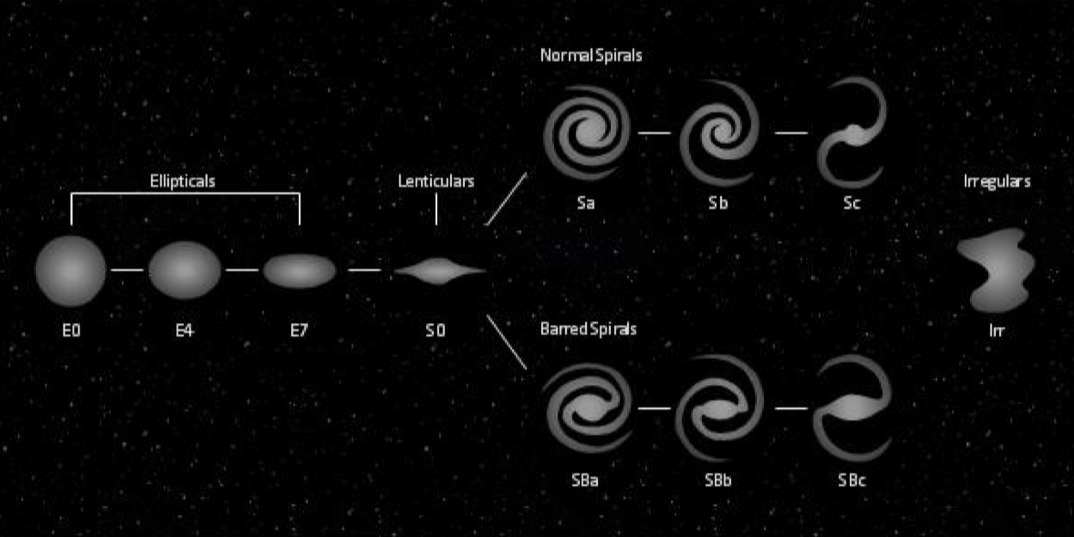
\includegraphics[width=12cm]{chapters/25/fork}
  \caption{星系类型的哈勃音叉形图}
  \label{fig:hubblesequence}
\end{figure}

\section{漩涡星系和不规则星系}
前面提到,可以用21\,cm线来探测气体的分布,因为计算表明其光深约等于中性氢的柱密度。由于它位于微波波段,不容易被星际介质散射,同时也能穿过地球大气,因此也是探测星系结构的很好工具。而通过21\,cm线的多普勒频移,我们还可以探测星系的运动情况。

\subsection{塔利-费希尔关系}
星系的气体受引力束缚转动,因此最大转动速度和中心质量存在一定关系,由于暗物质晕的存在且质量远大于星系质量,因此最大转动速度可以近似为常数,而对于所有漩涡星系,存在相同的质光比$M/L\equiv 1/C_\mathrm{ML}$,以及假设相同的表面亮度$L/R^2\equiv C_\mathrm{SB}$,我们可以得到星系光度和最大转动速度的关系:
\begin{equation}
  L={C_\mathrm{ML}^2\over C_\mathrm{SB}}{V_\mathrm{max}^4\over G^2}=CV_\mathrm{max}^4
\end{equation}

根据光度和星等的关系,可以将上式写为:
\begin{equation}
  M=-10\log_{10}V_\mathrm{max}+\mathrm{constant.}
\end{equation}

这种星系光度和最大旋转速度的关系最早在1977年被Tully和Fisher在观测上发现,也因此被命名为\textbf{塔利-费希尔关系}。

\subsection{超大质量黑洞}
通过对银河系中心处恒星的运动表明,银河系中心存在超大质量黑洞Sgr A*。对于其质量的测量,可以通过恒星运动轨迹来测定,但是还有一种方法是通过速度弥散来得到其维里质量。

前面说过引力束缚的平衡系统满足维里定理,即动能和引力势能存在确定关系,动能对应的就是速度,而观测上我们往往只能探测到速度的径向分量,并定义相关的速度弥散,因此我们可以通过速度弥散和维里定理来定义\textbf{维里质量}:
\begin{equation}
  M_\mathrm{virial}\approx{5R\sigma_r^2\over G}
\end{equation}

\subsection{漩涡结构}
关于漩涡星系的漩涡结构是如何形成的,有多种模型来解释,但是其中比较合理和广泛接受的是\textbf{密度波理论}。

这种理论认为漩涡星系的旋臂是气体压缩和恒星形成的波,在银盘中运动。气体从后面进入旋臂,被压缩,形成恒星。旋臂的形式由尘埃带、高气体密度区和新形成的OB恒星描绘。

更具体的解释是,如图\ref{fig:densitywave},由于不同半径的恒星的公转轨道并不是同轴的椭圆,而是存在一个相位差,相位差会导致旋转过程中恒星的密度分布会不同,从而形成了旋臂。

\begin{figure}[hbt]
  \centering
  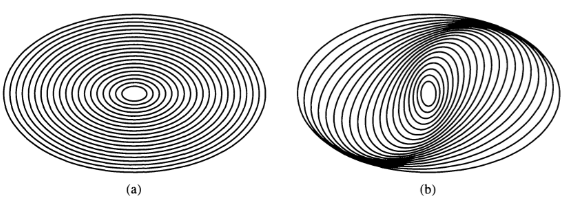
\includegraphics[width=10cm]{chapters/25/densitywave}
  \caption{密度波形成示意图。(a)正常同轴的恒星绕转椭圆轨道(b)彼此有一定夹角的恒星绕转椭圆轨道,可以形成双旋臂}
  \label{fig:densitywave}
\end{figure}

实际漩涡星系内的恒星当然不可能都具有如此理想的椭圆轨道,但却同样会形成这样的密度波旋臂。

\section{椭圆星系}
不像漩涡星系的气体有较统一的转动方向,对于椭圆星系来说,气体的速度弥散更高,因此无法具有漩涡星系那样的光度和最大旋转速度的关系。但是通过维里定理和一些简单假设,也可以得到椭圆星系光度和中心速度弥散的关系——\textbf{费伯-杰克逊关系}:
\begin{equation}
  L\propto\sigma_0^4
\end{equation}

\chapter{星系演化}
\section{星系的相互作用}
当两个星系相互``碰撞''时,实际上由于恒星间的距离较大,并不会发生真正的碰撞,但是引力的作用还是会发生。两个彼此擦肩而过的恒星之间的引力作用,会有把它们拉向彼此的趋势,这会造成恒星的运动速度会下降,而在更大的尺度上,这种普遍的速度下降会使星系的运动速度也下降。这种阻碍运动效果有点类似于摩擦力,因此被称为\textbf{动力学摩擦}:
\begin{equation}
  f_d\simeq C{G^2M^2\rho \over v_M^2}
\end{equation}

其中$C$是一个无量纲量,是星系速度$v_M$和速度弥散$\sigma$的比值。

\section{星系的形成}
\subsection{ELS塌缩模型}
过程和恒星形成类似,但是是尺度更大的星云快速塌缩形成的,这能够比较好的解释许多银晕中的年老恒星具有很高偏心率的椭圆轨道,因为它们在塌缩过程中就开始形成了,还保留了很大的塌缩带来的径向速度。

但是观测上有许多这种模型无法解释的现象
\begin{itemize}
  \item 一半外银晕的恒星具有逆行轨道,因此银晕的整体角速度接近0,与模型预测不符
  \item 球状星团和银晕年龄相差太大
  \item 球状星团的化学组成不统一
\end{itemize}

因此人们提出了一些新的模型来解释观测现象:
\paragraph{耗散塌缩模型}
考虑冷却时标比自由落体时标长,塌缩过程中温度会上升,塌缩速度会变慢

\paragraph{阶梯式并合模型}
通过吞并小星系成长,这会导致不同星系的成分会混合,这能够解释球状星团年龄和金属丰度的差异。近期的高红移观测支持了这一模型,他们的观测发现高红移区(代表很久之前)具有比现在更多数量的小星系。

\chapter{宇宙的结构}
\section{系外距离测量}
如果距离的尺度大于银河系的尺度时,这时就被称为系外距离尺度或\textbf{宇宙学距离尺度}(Mpc量级)。对于这种尺度的距离测量,三角视差的误差会比较大,因此需要引入其他的测距方法,其中最著名的称为\textbf{标准烛光}。标准烛光指的是一类我们已知光度的天体,而通过测量它们的视星等,我们就可以得到它们的距离。

\paragraph{造父变星}
由于造父变星具有周光关系,当我们测量到它的周期,也就意味着知道了它的光度
\begin{equation}
  M_{\langle V\rangle}=-3.53\log_{10}P_d-2.13+2.13(B-V)
\end{equation}

目前观测到的最远造父变星可以达29\,Mpc。

\paragraph{Ia型超新星}
前面提到Ia型超新星的产生是由于白矮星吸积物质达到了钱德拉塞卡极限,因此爆发时具有一个统一的光度。\mbox{}\\

其他的能够用于距离探测的\textbf{示距天体}还包括:新星(20\,Mpc)、最亮的红巨星(7\,Mpc)、球状星团、行星状星云和塔利-费希尔关系等。

\section{宇宙的膨胀}
\textbf{哈勃定律}告诉我们所有的星系都是在远离我们运动的,并且退行速度和距离成正比
\begin{equation}
  v=H_0d
\end{equation}

其中$H_0=100h\;\mathrm{km\,s^{-1}\,Mpc^{-1}}$是\textbf{哈勃常数},$h$的取值范围是0.5-1;现在通常取0.7,这显然也可以作为测距方式。哈勃定律还解释的一个现象则是宇宙的空间是在加速膨胀的,星系随着空间膨胀的运动被称之为\textbf{哈伯流},而引力束缚系统不随空间发生膨胀。

\paragraph{大爆炸理论}
如果宇宙是在膨胀,那么倒过来考虑,一开始宇宙应该只是一个奇点,之后一切的物质都起源于一场大爆炸,宇宙开始膨胀。而早期的宇宙温度非常高,充满了黑体辐射,随着宇宙的膨胀,温度逐渐降低,辐射峰值也会随之红移,最终变成了现在的微波波段的\textbf{宇宙微波背景}(cosmic microwave background),对应温度3\;K。














\end{document}